%%%%%%%%%%%%%%%%%%%%%%%%%%%%%%%%%%%%%%%%%%%%%%%%%%%%%%%%%%%%
%%  This Beamer template was created by Cameron Bracken.
%%  Anyone can freely use or modify it for any purpose
%%  without attribution.
%%
%%  Last Modified: January 9, 2009
%%

\documentclass[xcolor=x11names,compress]{beamer}

%% General document %%%%%%%%%%%%%%%%%%%%%%%%%%%%%%%%%%
\usepackage{graphicx}
\usepackage{tikz}
\usepackage{graphicx}
\usepackage{amsmath}

\usetikzlibrary{decorations.fractals}
%%%%%%%%%%%%%%%%%%%%%%%%%%%%%%%%%%%%%%%%%%%%%%%%%%%%%%


%% Beamer Layout %%%%%%%%%%%%%%%%%%%%%%%%%%%%%%%%%%
\useoutertheme[subsection=false,shadow]{miniframes}
\useinnertheme{default}
\usefonttheme{serif}
\usepackage{palatino}

\setbeamerfont{title like}{shape=\scshape}
\setbeamerfont{frametitle}{shape=\scshape}

\setbeamercolor*{lower separation line head}{bg=DeepSkyBlue4} 
\setbeamercolor*{normal text}{fg=black,bg=white} 
\setbeamercolor*{alerted text}{fg=red} 
\setbeamercolor*{example text}{fg=black} 
\setbeamercolor*{structure}{fg=black} 

\setbeamercolor*{palette tertiary}{fg=black,bg=black!10} 
\setbeamercolor*{palette quaternary}{fg=black,bg=black!10} 

\renewcommand{\(}{\begin{columns}}
\renewcommand{\)}{\end{columns}}
\newcommand{\<}[1]{\begin{column}{#1}}
\renewcommand{\>}{\end{column}}
%%%%%%%%%%%%%%%%%%%%%%%%%%%%%%%%%%%%%%%%%%%%%%%%%%


\begin{document}


%%%%%%%%%%%%%%%%%%%%%%%%%%%%%%%%%%%%%%%%%%%%%%%%%%%%%%

\begin{frame}
\title{QSEP Research Update}
%\subtitle{SUBTITLE}
\author{
	Halley Brantley\\
	{\it Savvy Sherpa}\\
}
\date{
	\begin{tikzpicture}[decoration=Koch curve type 2] 
	\draw[DeepSkyBlue4] decorate{ decorate{ decorate{ (0,0) -- (3,0) }}}; 
	\end{tikzpicture}  
	\\
	\vspace{1cm}
	\today
}
\titlepage
\end{frame}

\section{\scshape Overview}

\begin{frame}{Research Questions}
\begin{itemize}
	\item Can we identify a dataset containing the pediatric illness populations of interest and their immediate family members? 
	\item Can we quantify the outcomes of interest and their relationship to the hypothesized mediating factors? 
	\item Do we see any significant secondary effects of pediatric illness on family members, in comparison to a sensibly-defined control group? 
\end{itemize}
\end{frame}

\section{\scshape Data}

\begin{frame}{Dataset - from data team}
\begin{itemize}
	\item Count of sick children (under 24) in our dataset:  286,836
	\item Total member count (family members \& sick children combined): 973,718
	\item Total family count: 249,249
	\item Dataset covers year 2014-2016 and includes months since diagnosis. 
	\item Between 65-70\% of members in each year were enrolled for 12 months
\end{itemize}
\end{frame}

\begin{frame}{Number of Children Under 16 with each condition}
\begin{itemize}
	\item Total sick children under 16: 194,108
	\item Autism (ASD): 13,708 
	\item Type 1 Diabetes (T1D): 2,612
	\item Cerebral Palsy: 2,197
	\item Asthma: 119,299
	\item Cancer: 36,347
	\item Traumatic Event: 34,963
	\item Multiple Conditions: 14,202
\end{itemize}	
\end{frame}

\begin{frame}{Data Cleaning }
\begin{itemize}
	\item Removed spend for members who were enrolled 3 months or less in a given year. 
	\item Want to look at just sick children under 16, and adults in the same household between 30 to 55. 
	\item Typically 1 or 2 members per household that meet these criteria, although several households have 3. 
\end{itemize}
\end{frame}

\section{\scshape Exploratory Analysis}

\begin{frame}{Asthma - Sick Child Spending}
\small
Outliers not shown. Blue lines represent median and 75 percentile of spend before diagnosis. Numbers
shown are number of member months included in boxplot. 
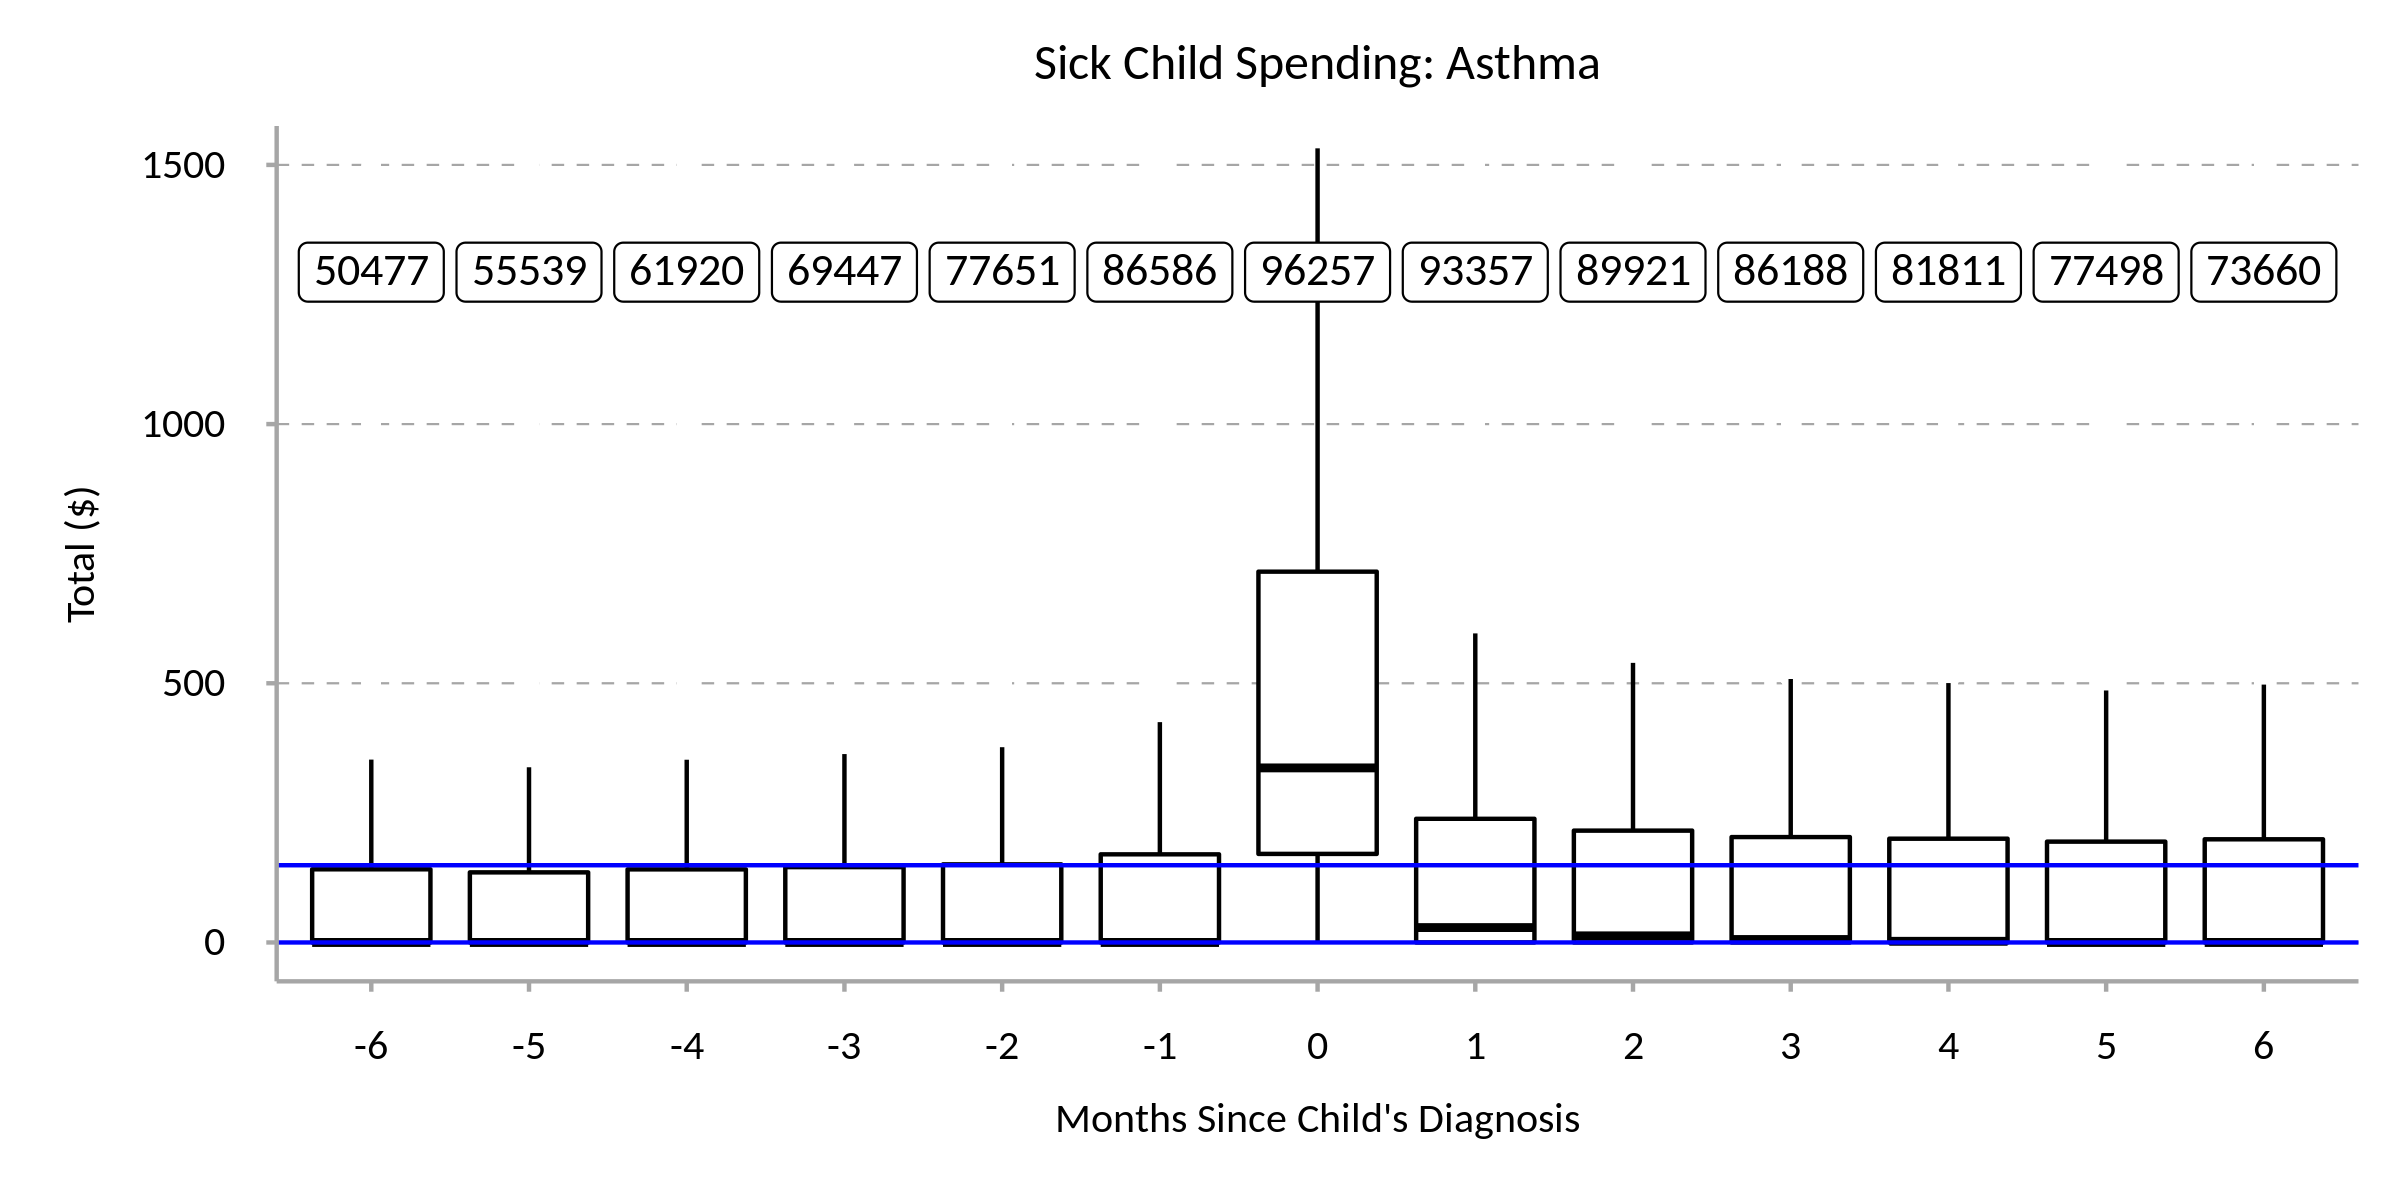
\includegraphics[width=\linewidth]{../figures/sick_child_spend_Asthma.png}
\end{frame}

\begin{frame}{Asthma - Adult Spending}
\small
Outliers not shown. Blue lines represent median and 75 percentile of spend before diagnosis. Numbers
shown are number of member months included in boxplot. 
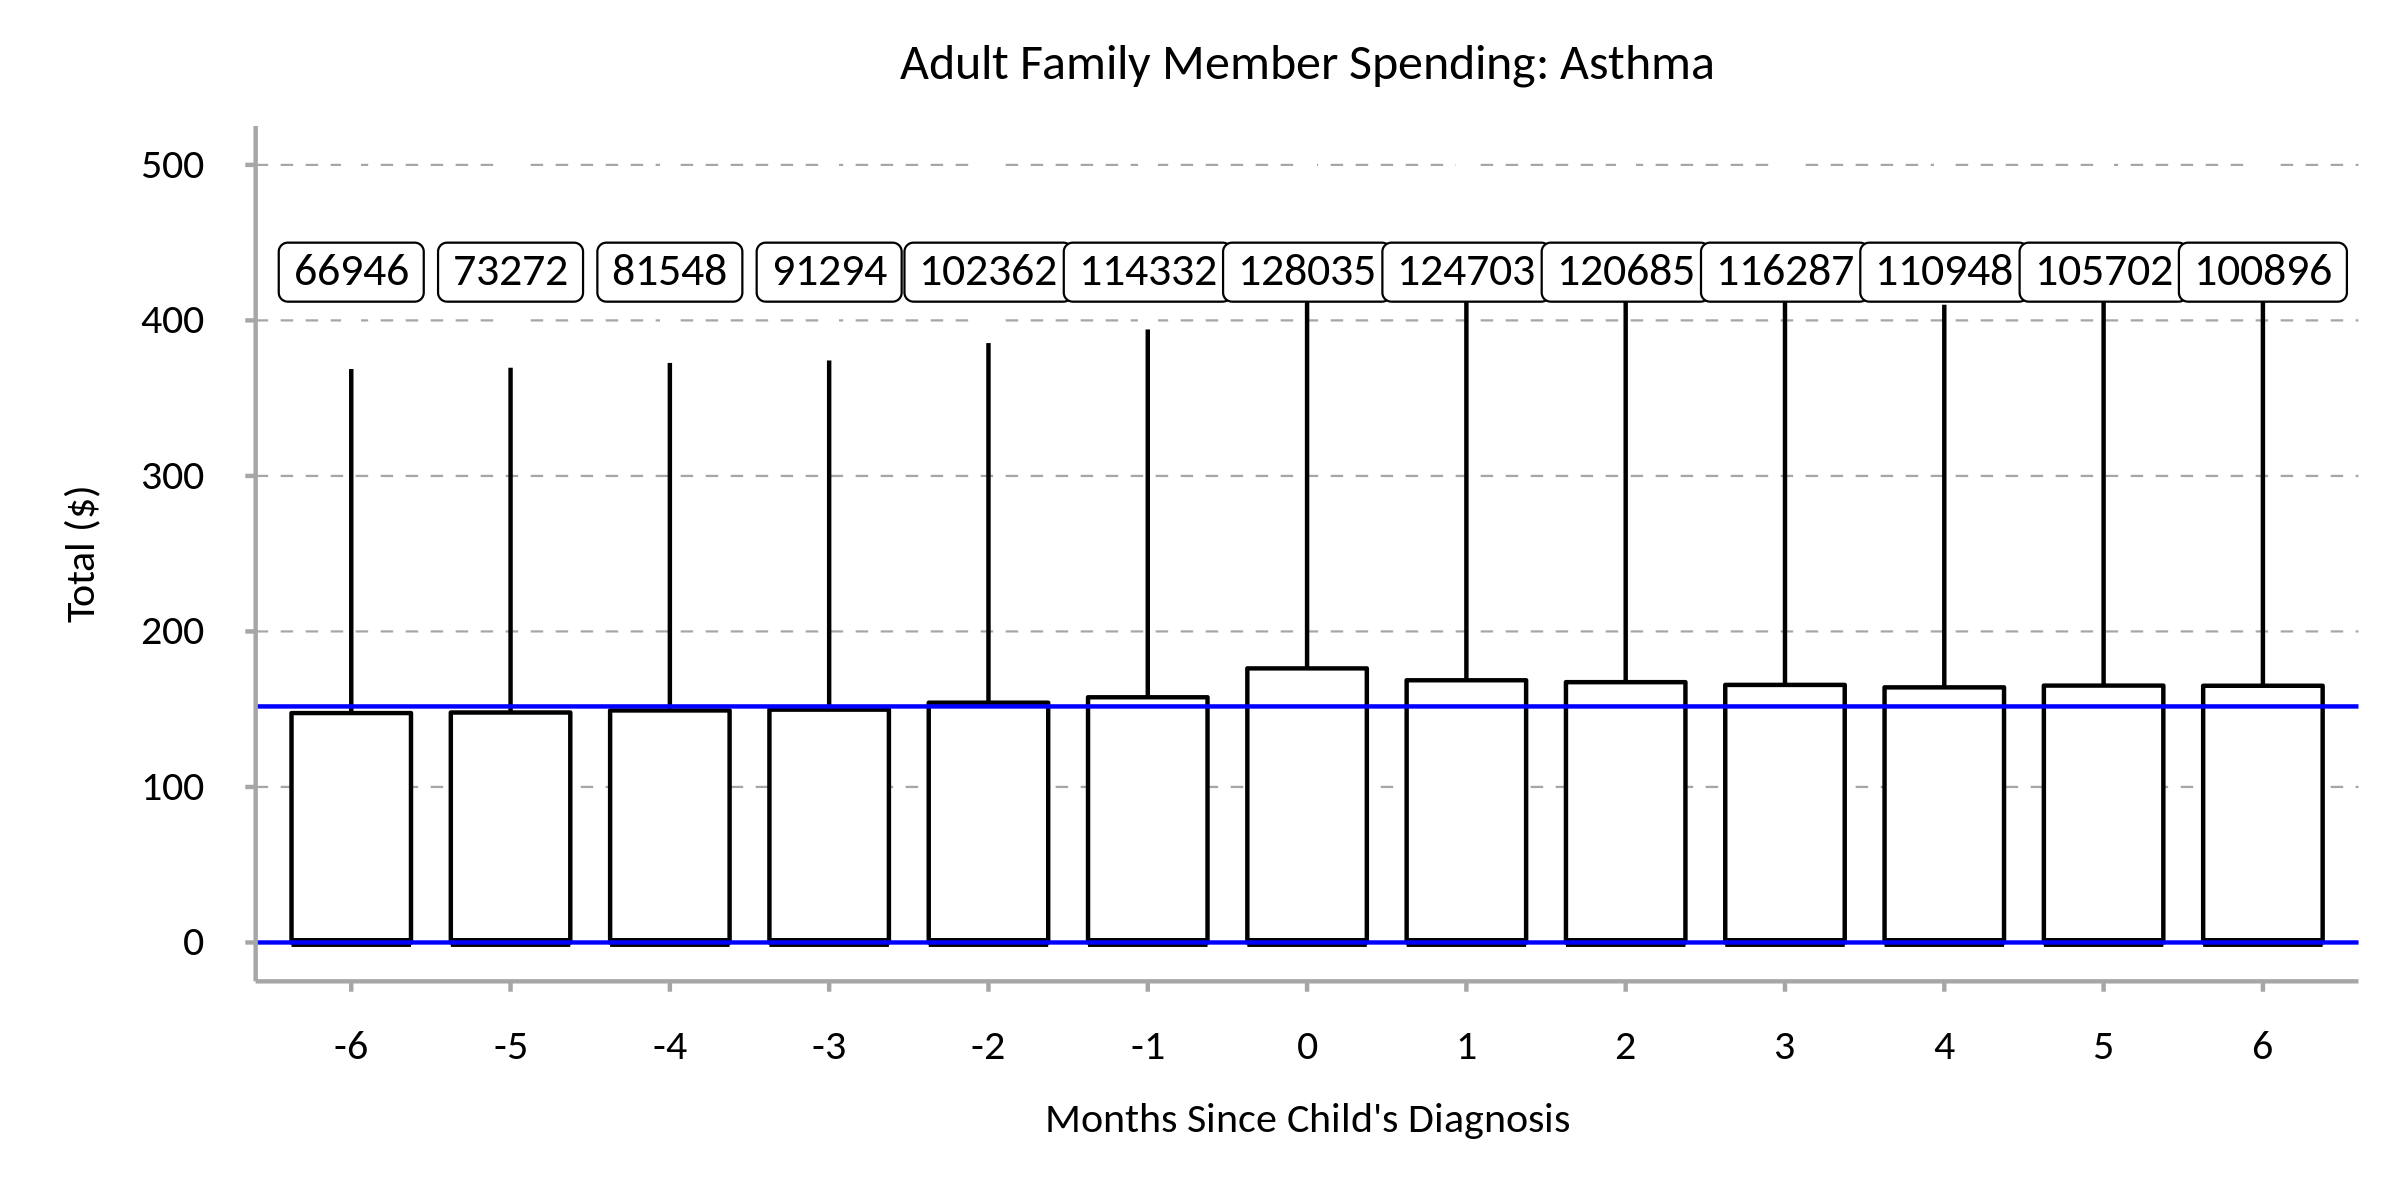
\includegraphics[width=\linewidth]{../figures/adult_family_spend_Asthma.png}
\end{frame}

\begin{frame}{Autism - Sick Child Spending}
\small
Outliers not shown. Blue lines represent median and 75 percentile of spend before diagnosis. Numbers
shown are number of member months included in boxplot. 
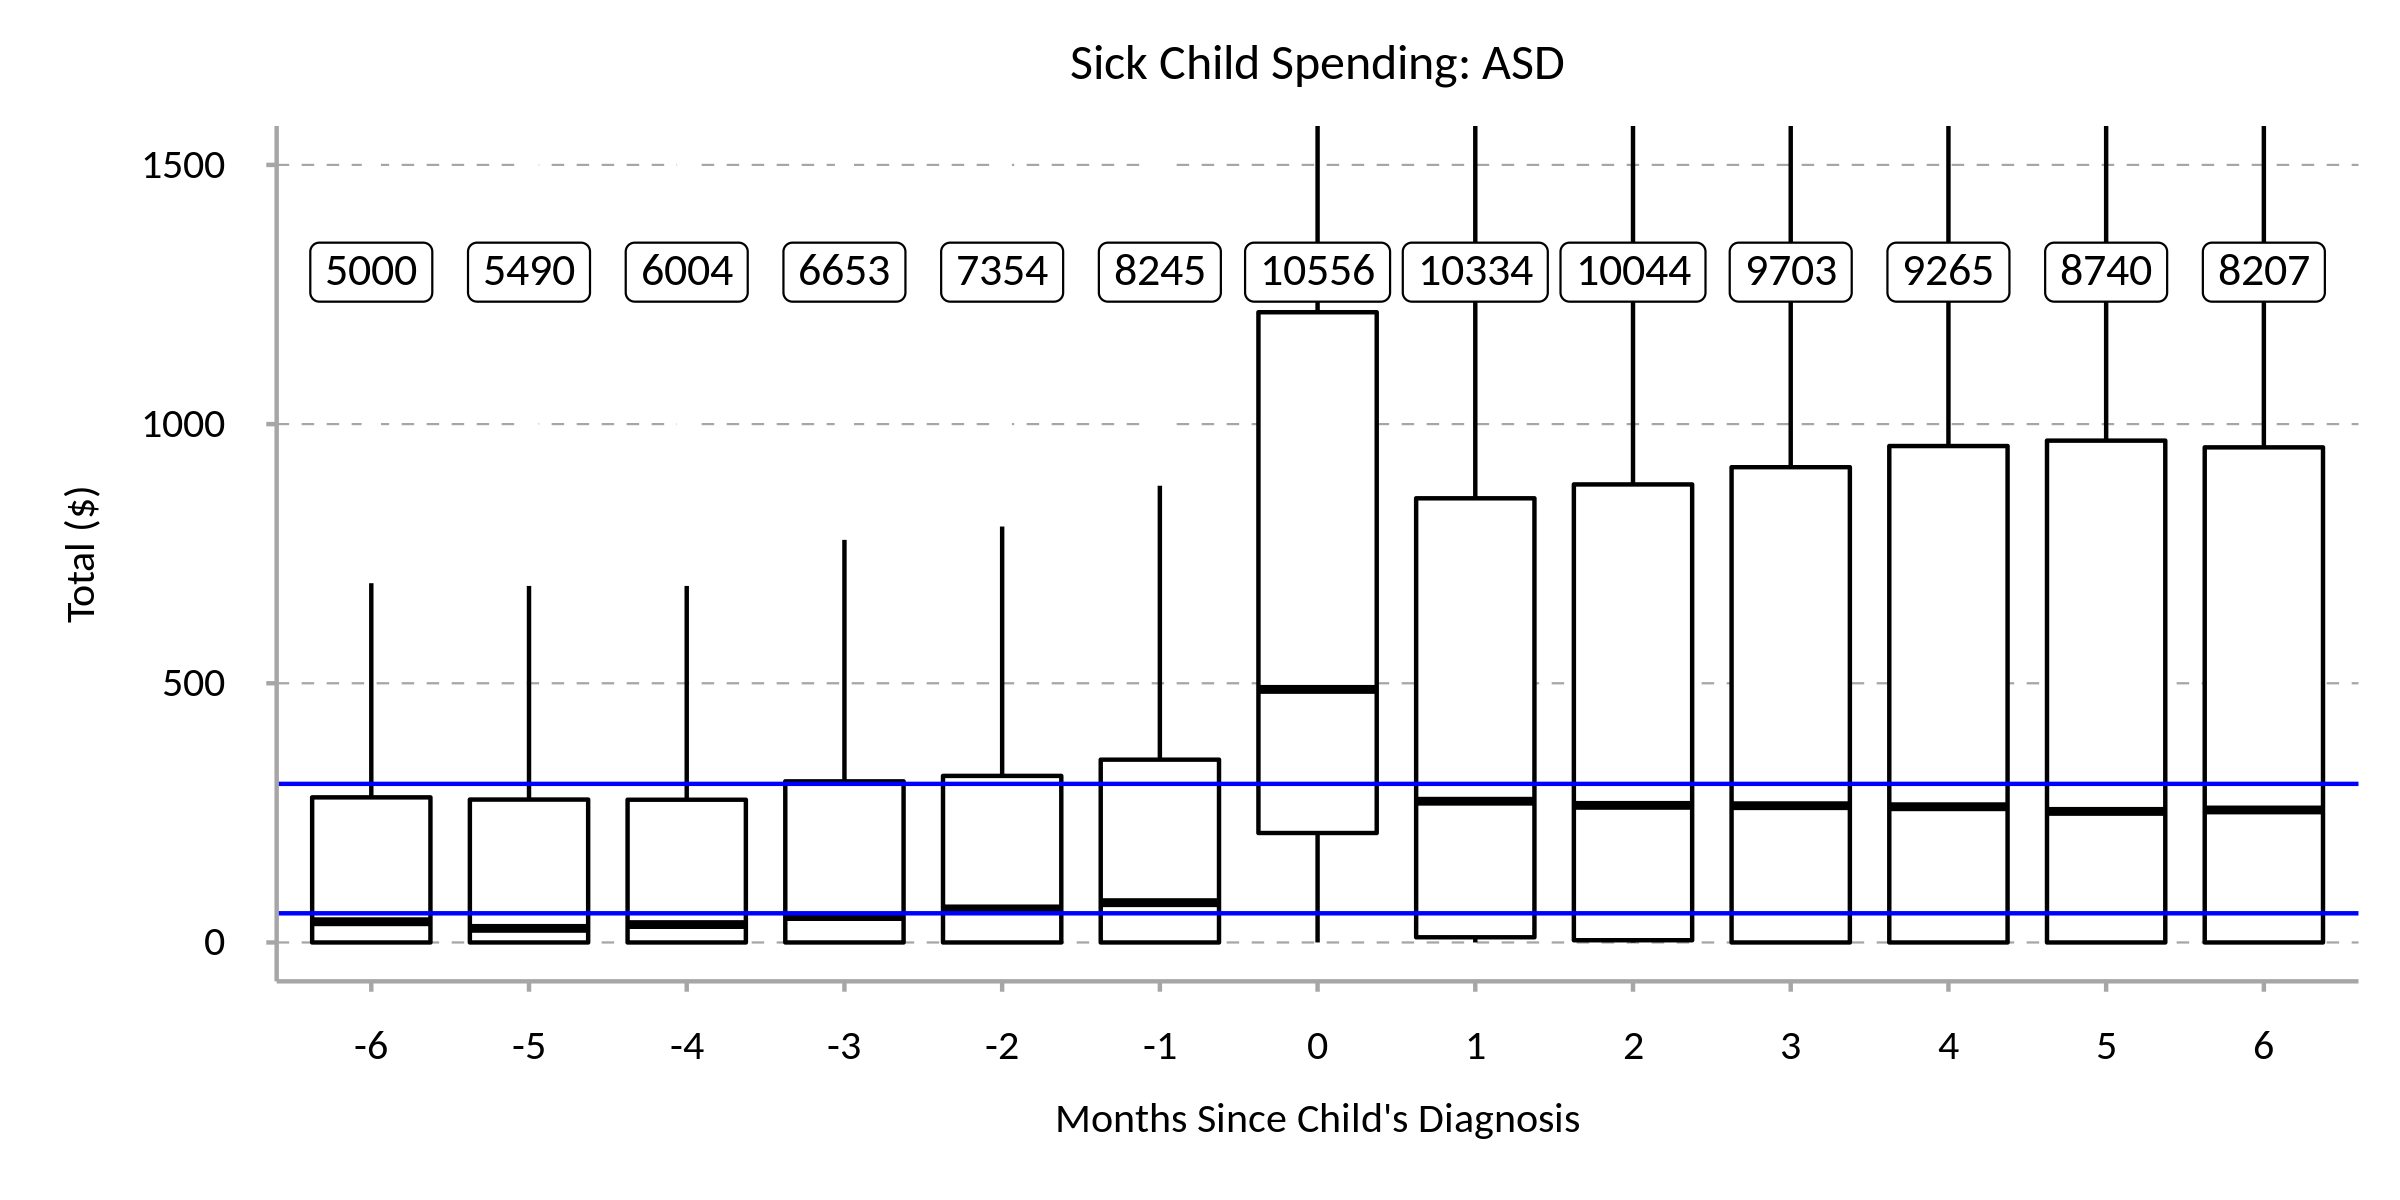
\includegraphics[width=\linewidth]{../figures/sick_child_spend_ASD.png}
\end{frame}

\begin{frame}{Autism - Adult Spending}
\small
Outliers not shown. Blue lines represent median and 75 percentile of spend before diagnosis. Numbers
shown are number of member months included in boxplot. 
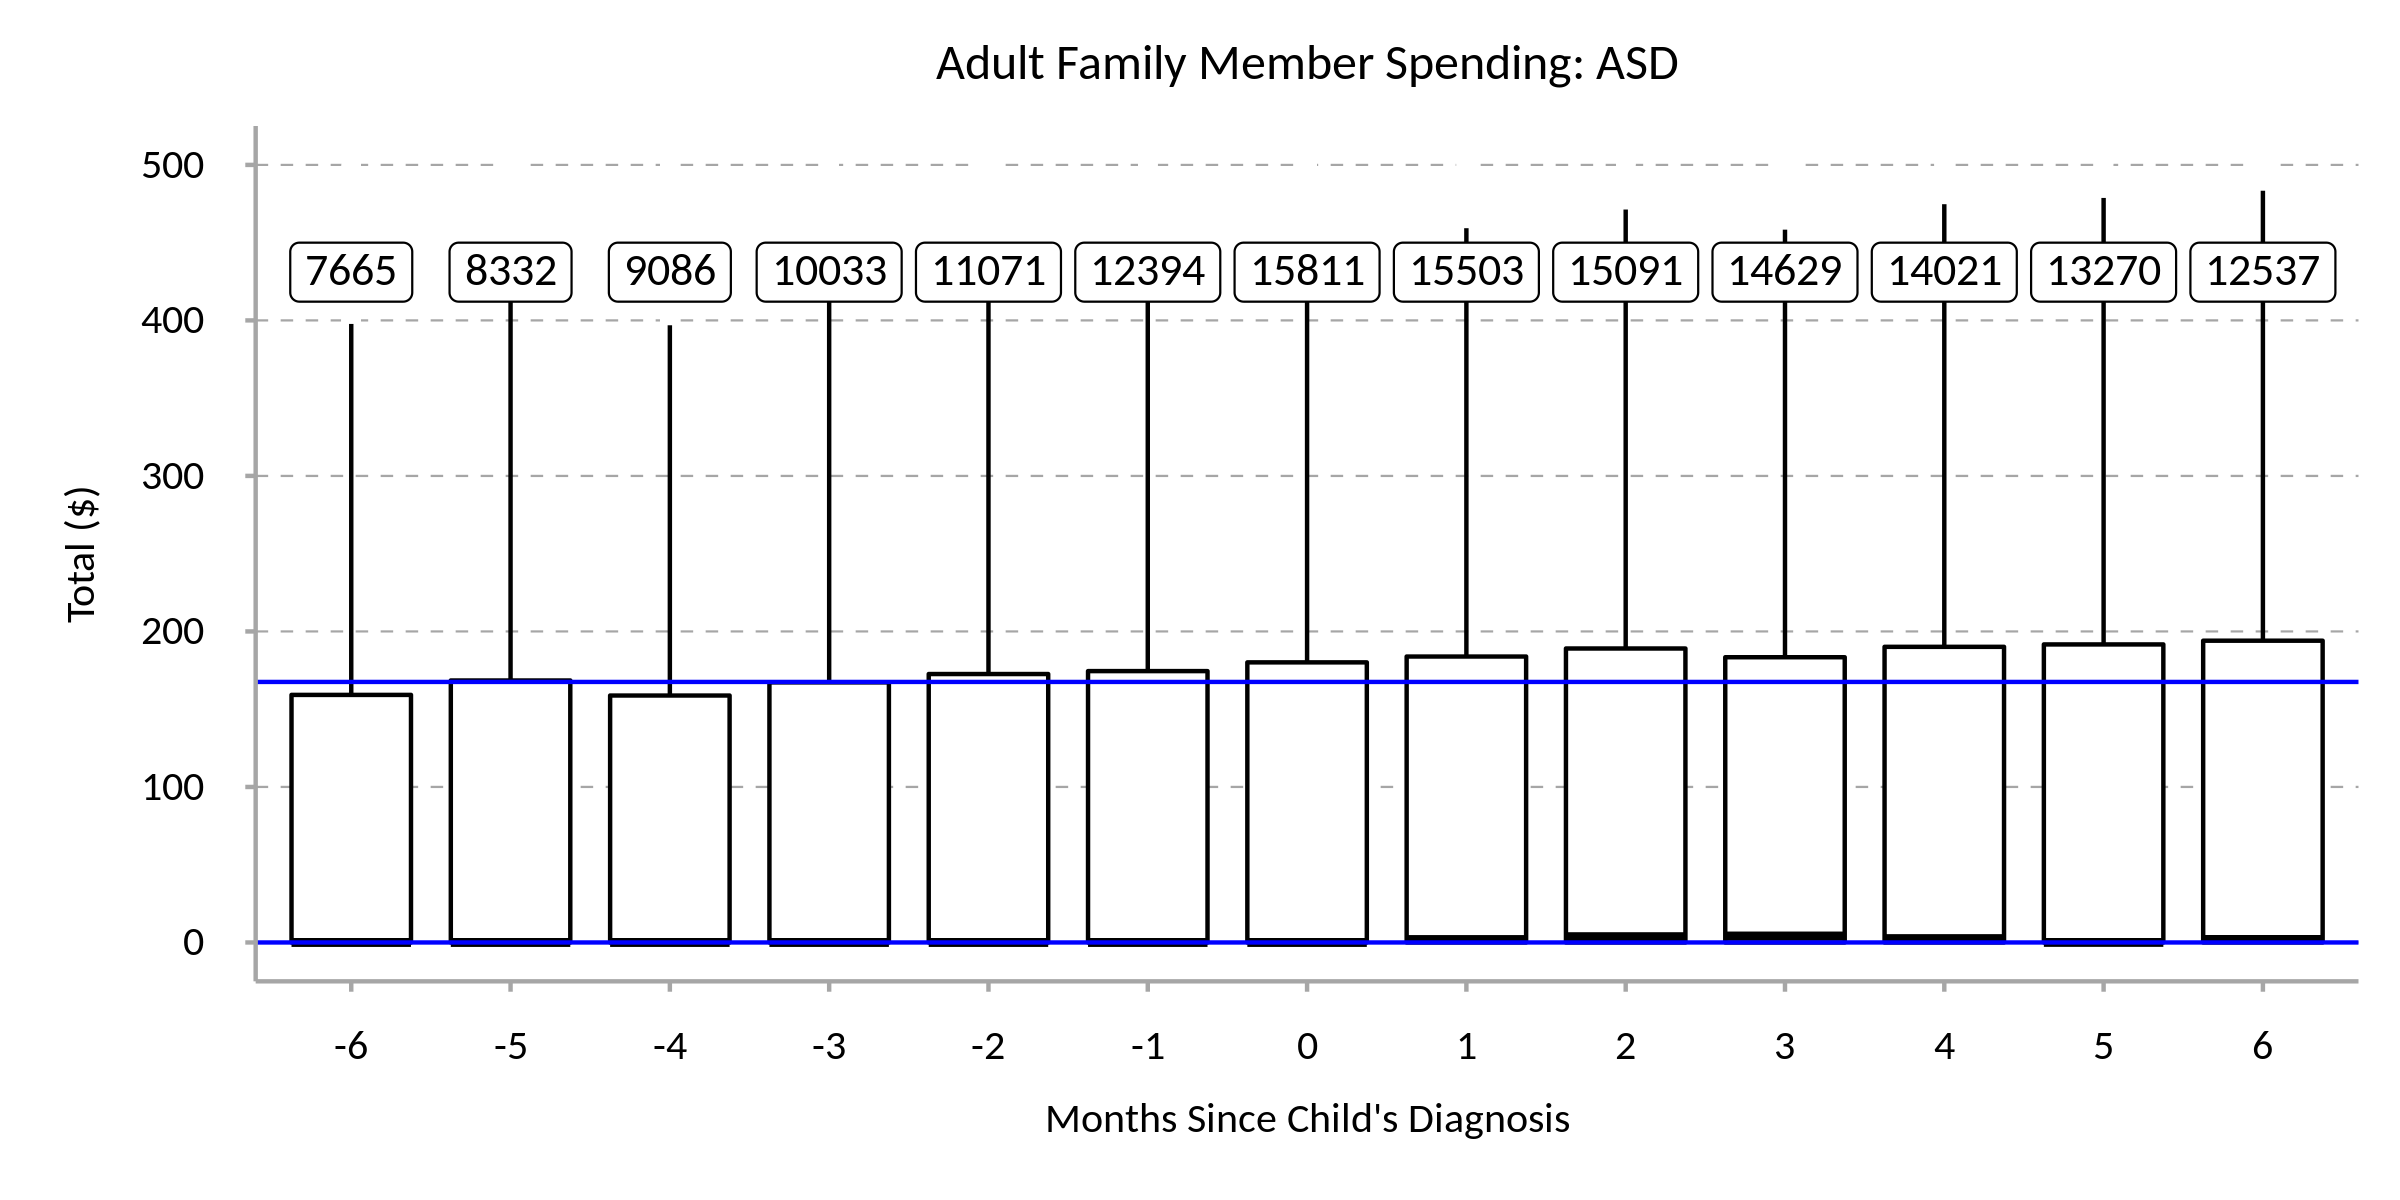
\includegraphics[width=\linewidth]{../figures/adult_family_spend_ASD.png}
\end{frame}

\begin{frame}{Cancer - Sick Child Spending}
\small
Outliers not shown. Blue lines represent median and 75 percentile of spend before diagnosis. Numbers
shown are number of member months included in boxplot. 
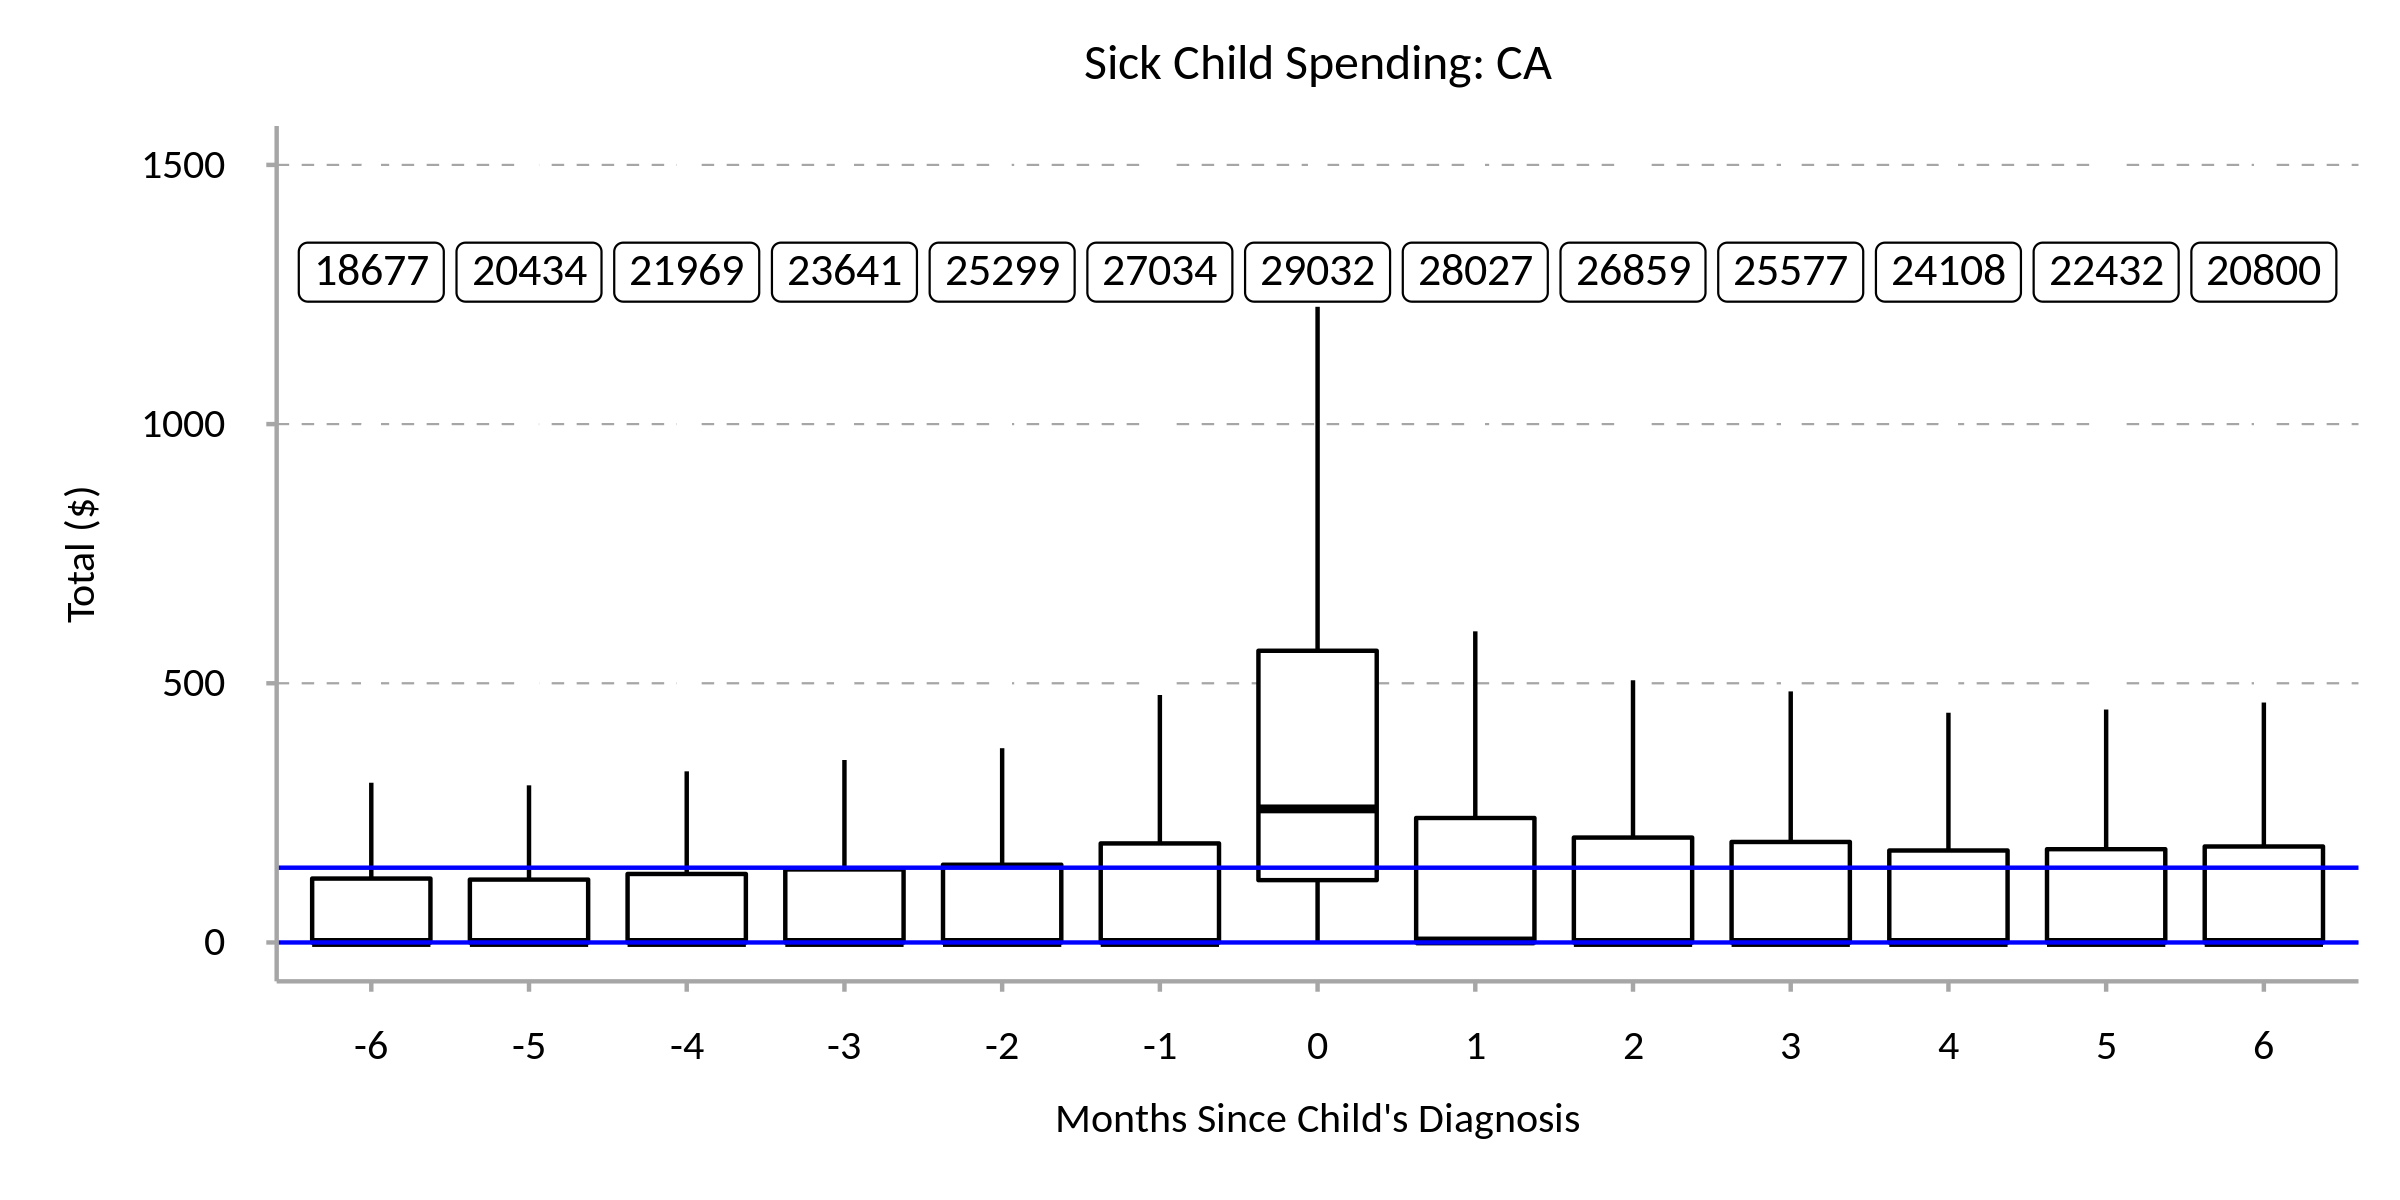
\includegraphics[width=\linewidth]{../figures/sick_child_spend_CA.png}
\end{frame}

\begin{frame}{Cancer - Adult Spending}
\small
Outliers not shown. Blue lines represent median and 75 percentile of spend before diagnosis. Numbers
shown are number of member months included in boxplot. 
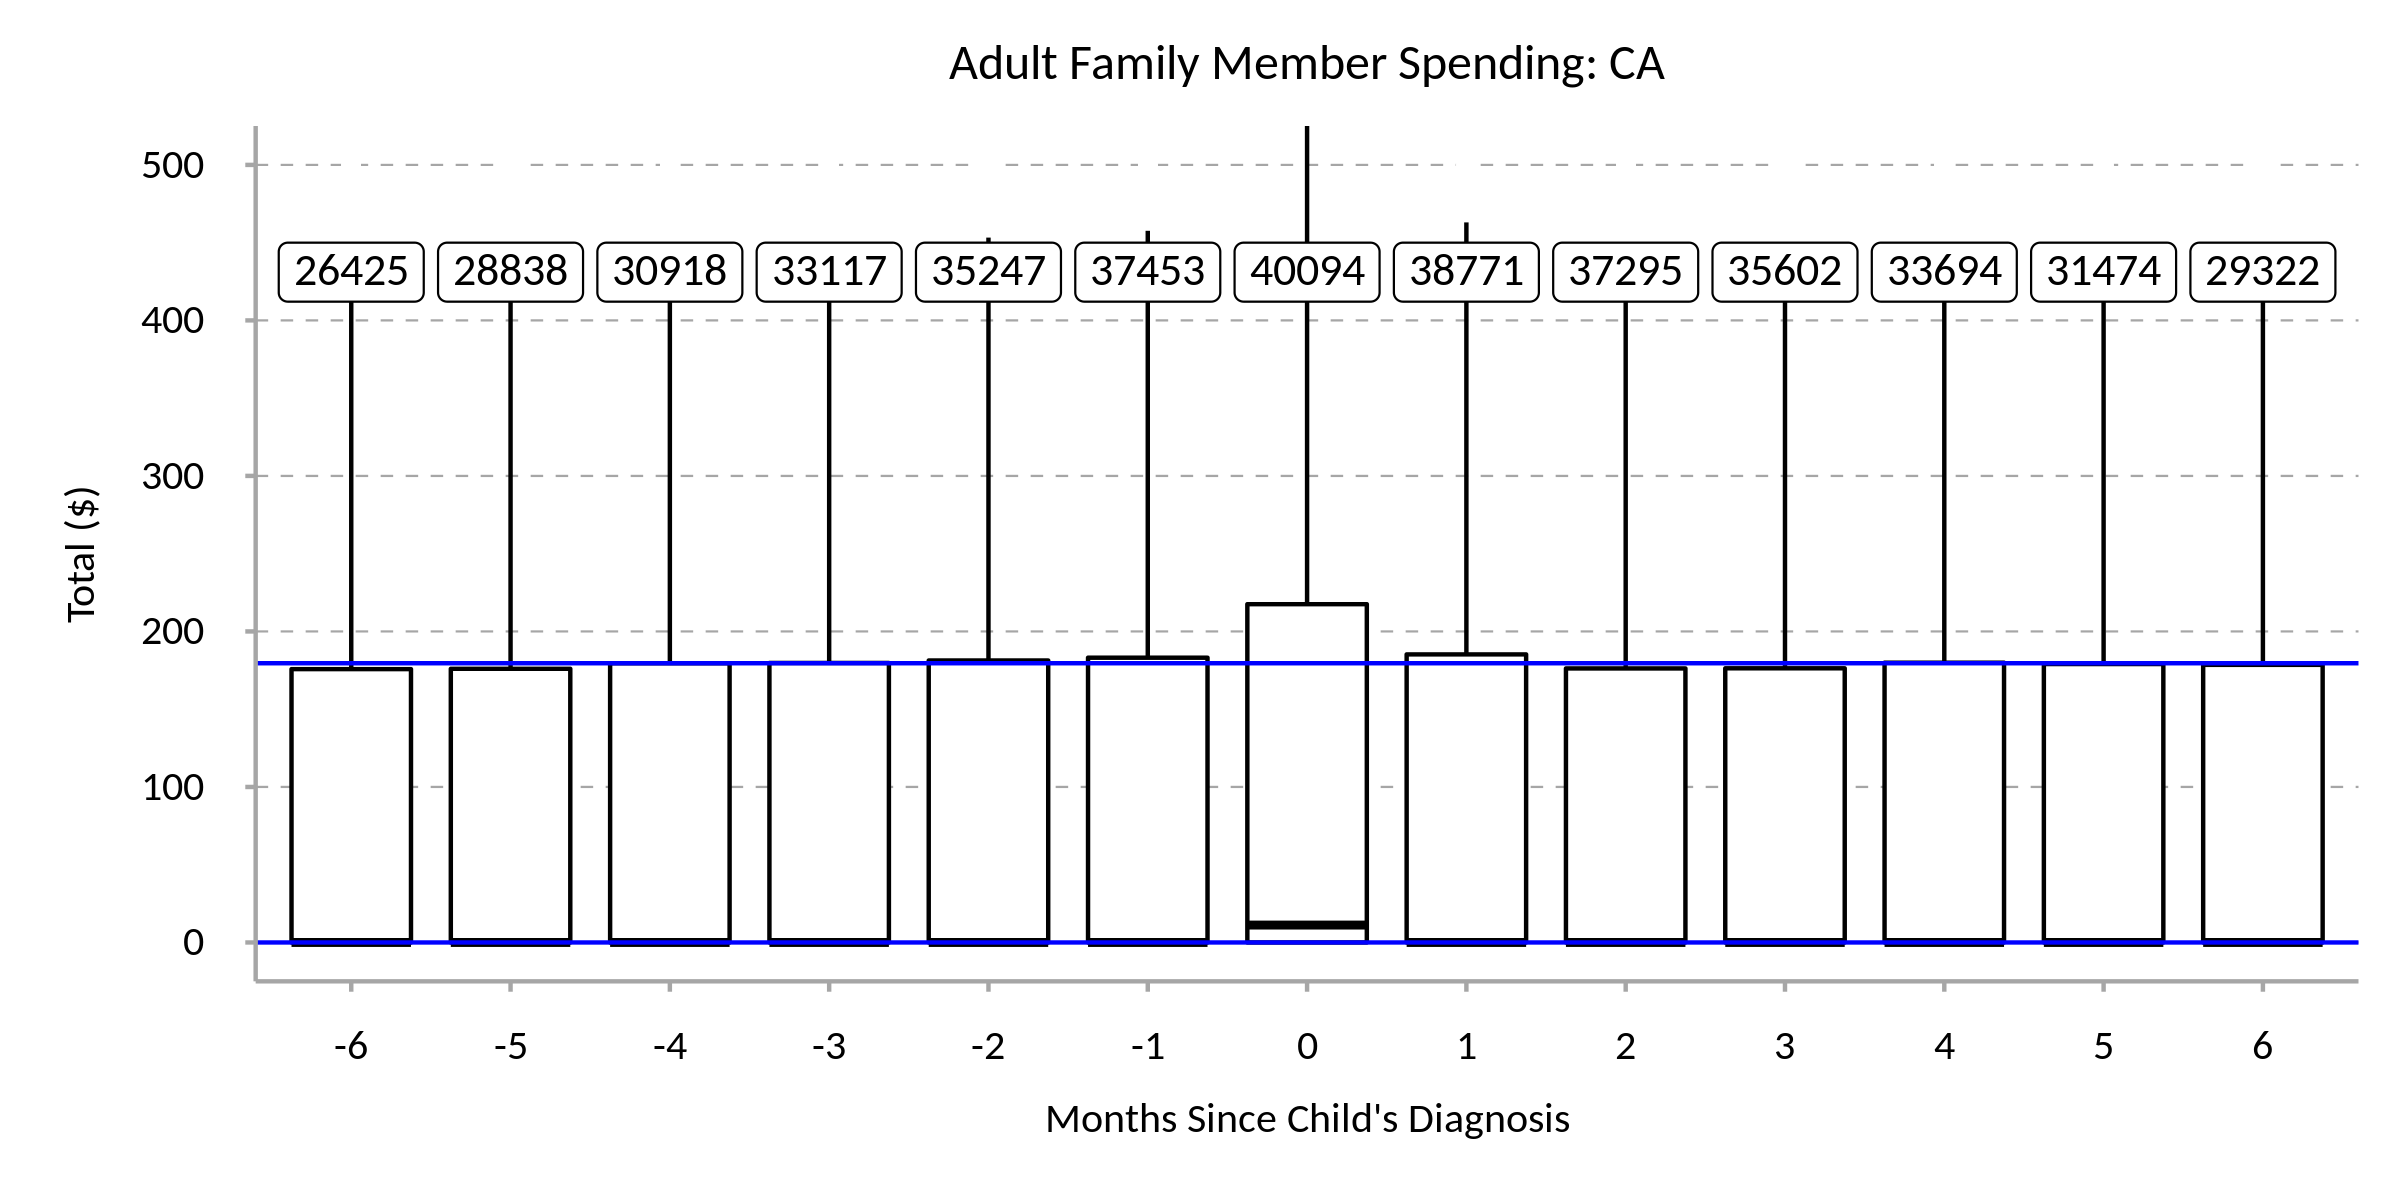
\includegraphics[width=\linewidth]{../figures/adult_family_spend_CA.png}
\end{frame}

\begin{frame}{Cerebral Palsy - Sick Child Spending}
\small
Outliers not shown. Blue lines represent median and 75 percentile of spend before diagnosis. Numbers
shown are number of member months included in boxplot. 
\includegraphics[width=\linewidth]{../figures/sick_child_spend_cerebral.png}
\end{frame}

\begin{frame}{Cerebral Palsy - Adult Spending}
\small
Outliers not shown. Blue lines represent median and 75 percentile of spend before diagnosis. Numbers
shown are number of member months included in boxplot. 
\includegraphics[width=\linewidth]{../figures/adult_family_spend_cerebral.png}
\end{frame}

\begin{frame}{Type 1 Diabetes - Sick Child Spending}
\small
Outliers not shown. Blue lines represent median and 75 percentile of spend before diagnosis. Numbers
shown are number of member months included in boxplot. 
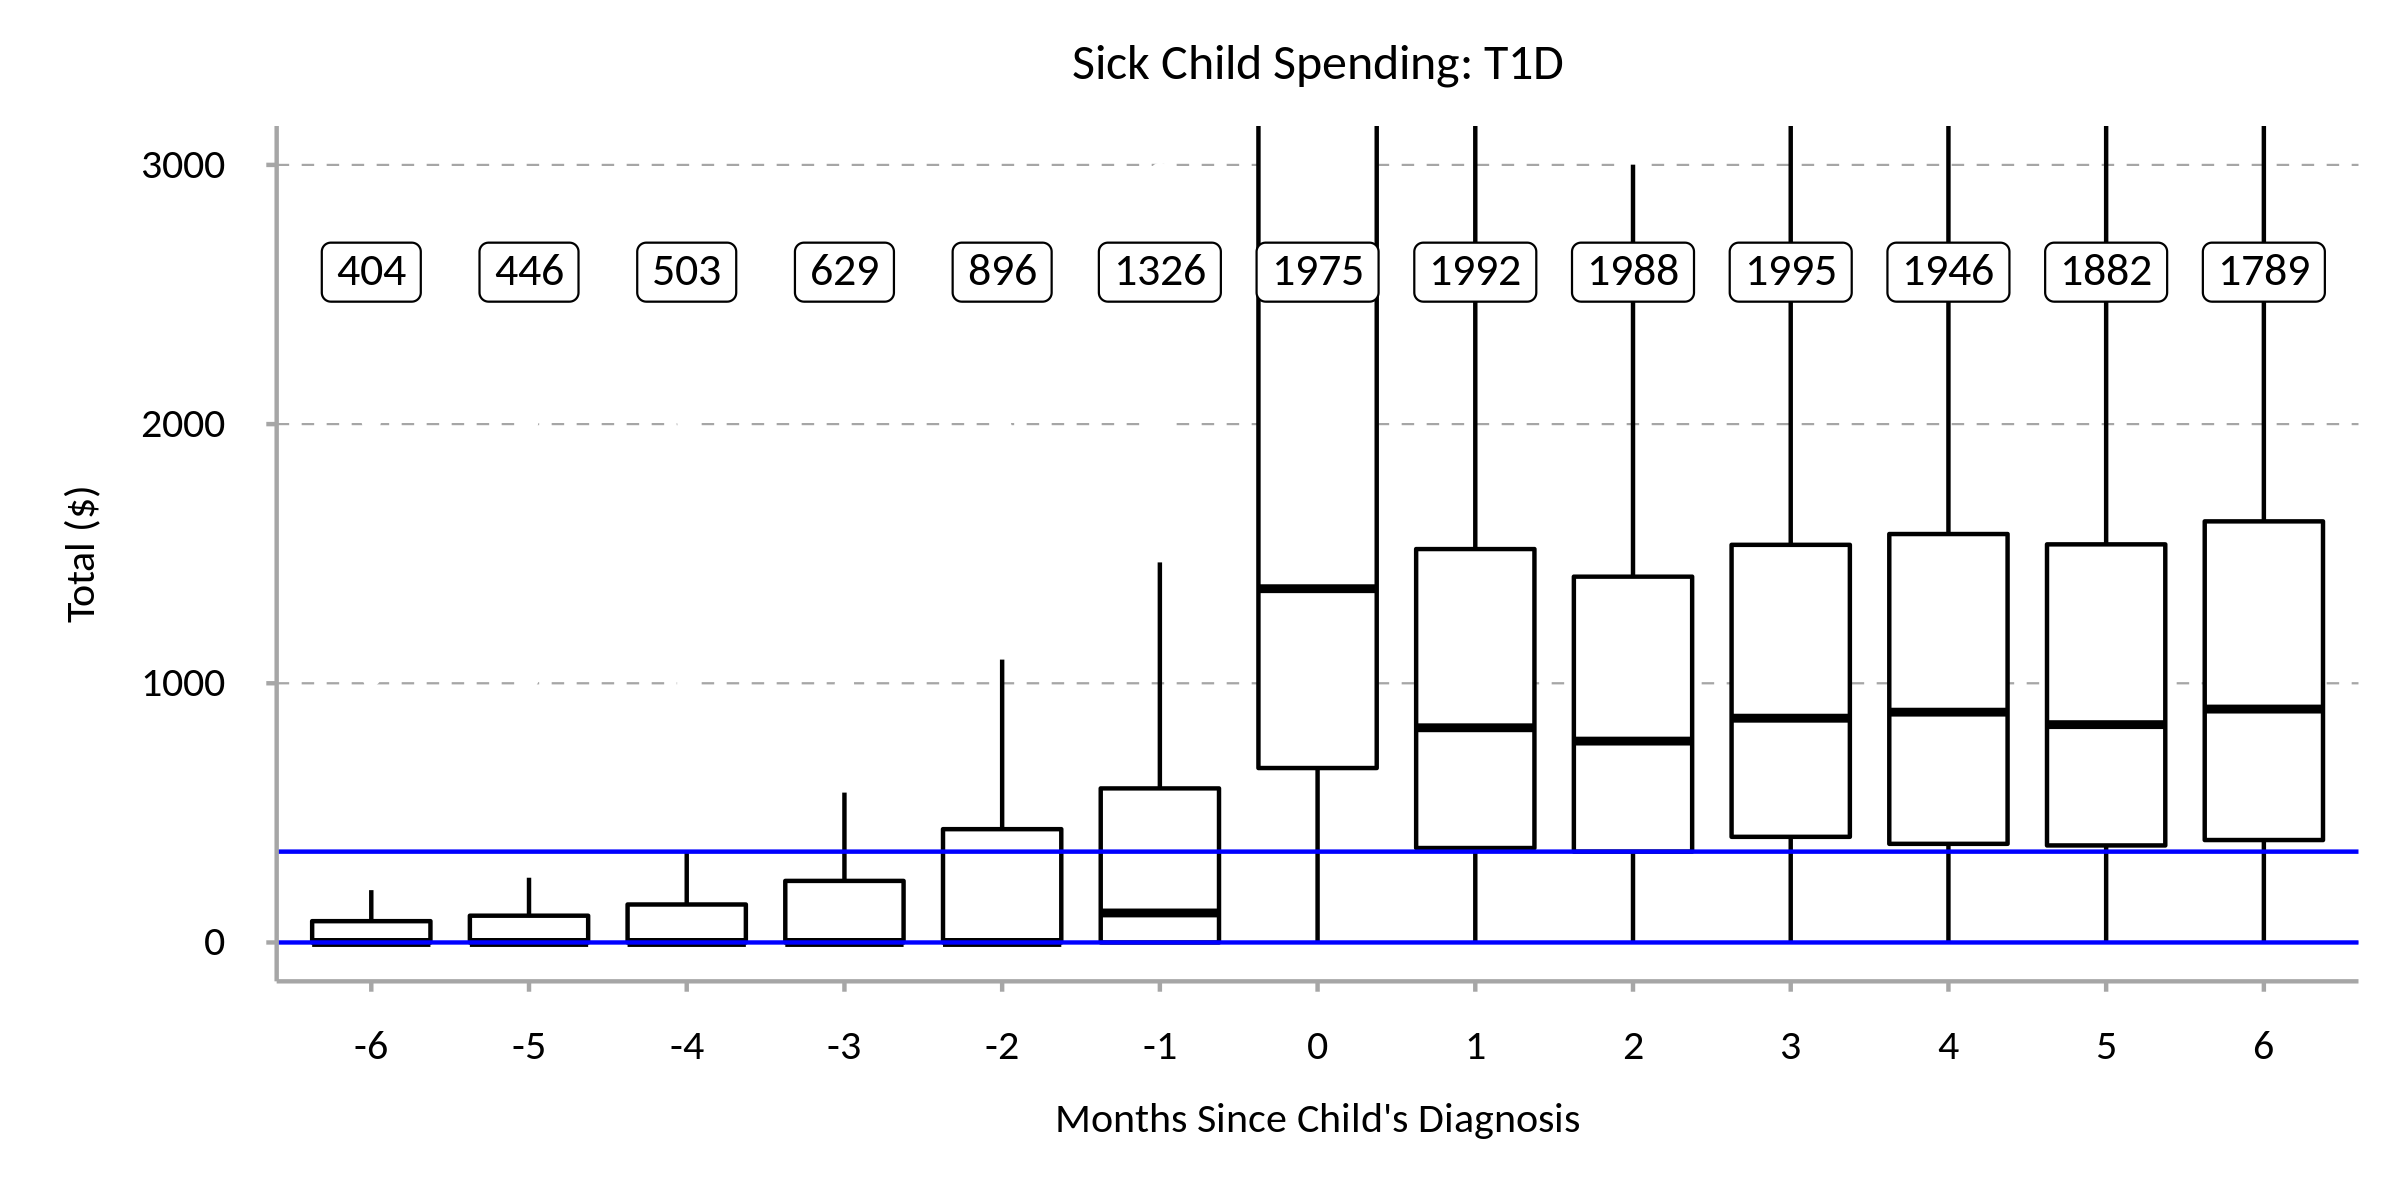
\includegraphics[width=\linewidth]{../figures/sick_child_spend_T1D.png}
\end{frame}

\begin{frame}{Type 1 Diabetes - Adult Spending}
\small
Outliers not shown. Blue lines represent median and 75 percentile of spend before diagnosis. Numbers
shown are number of member months included in boxplot. 
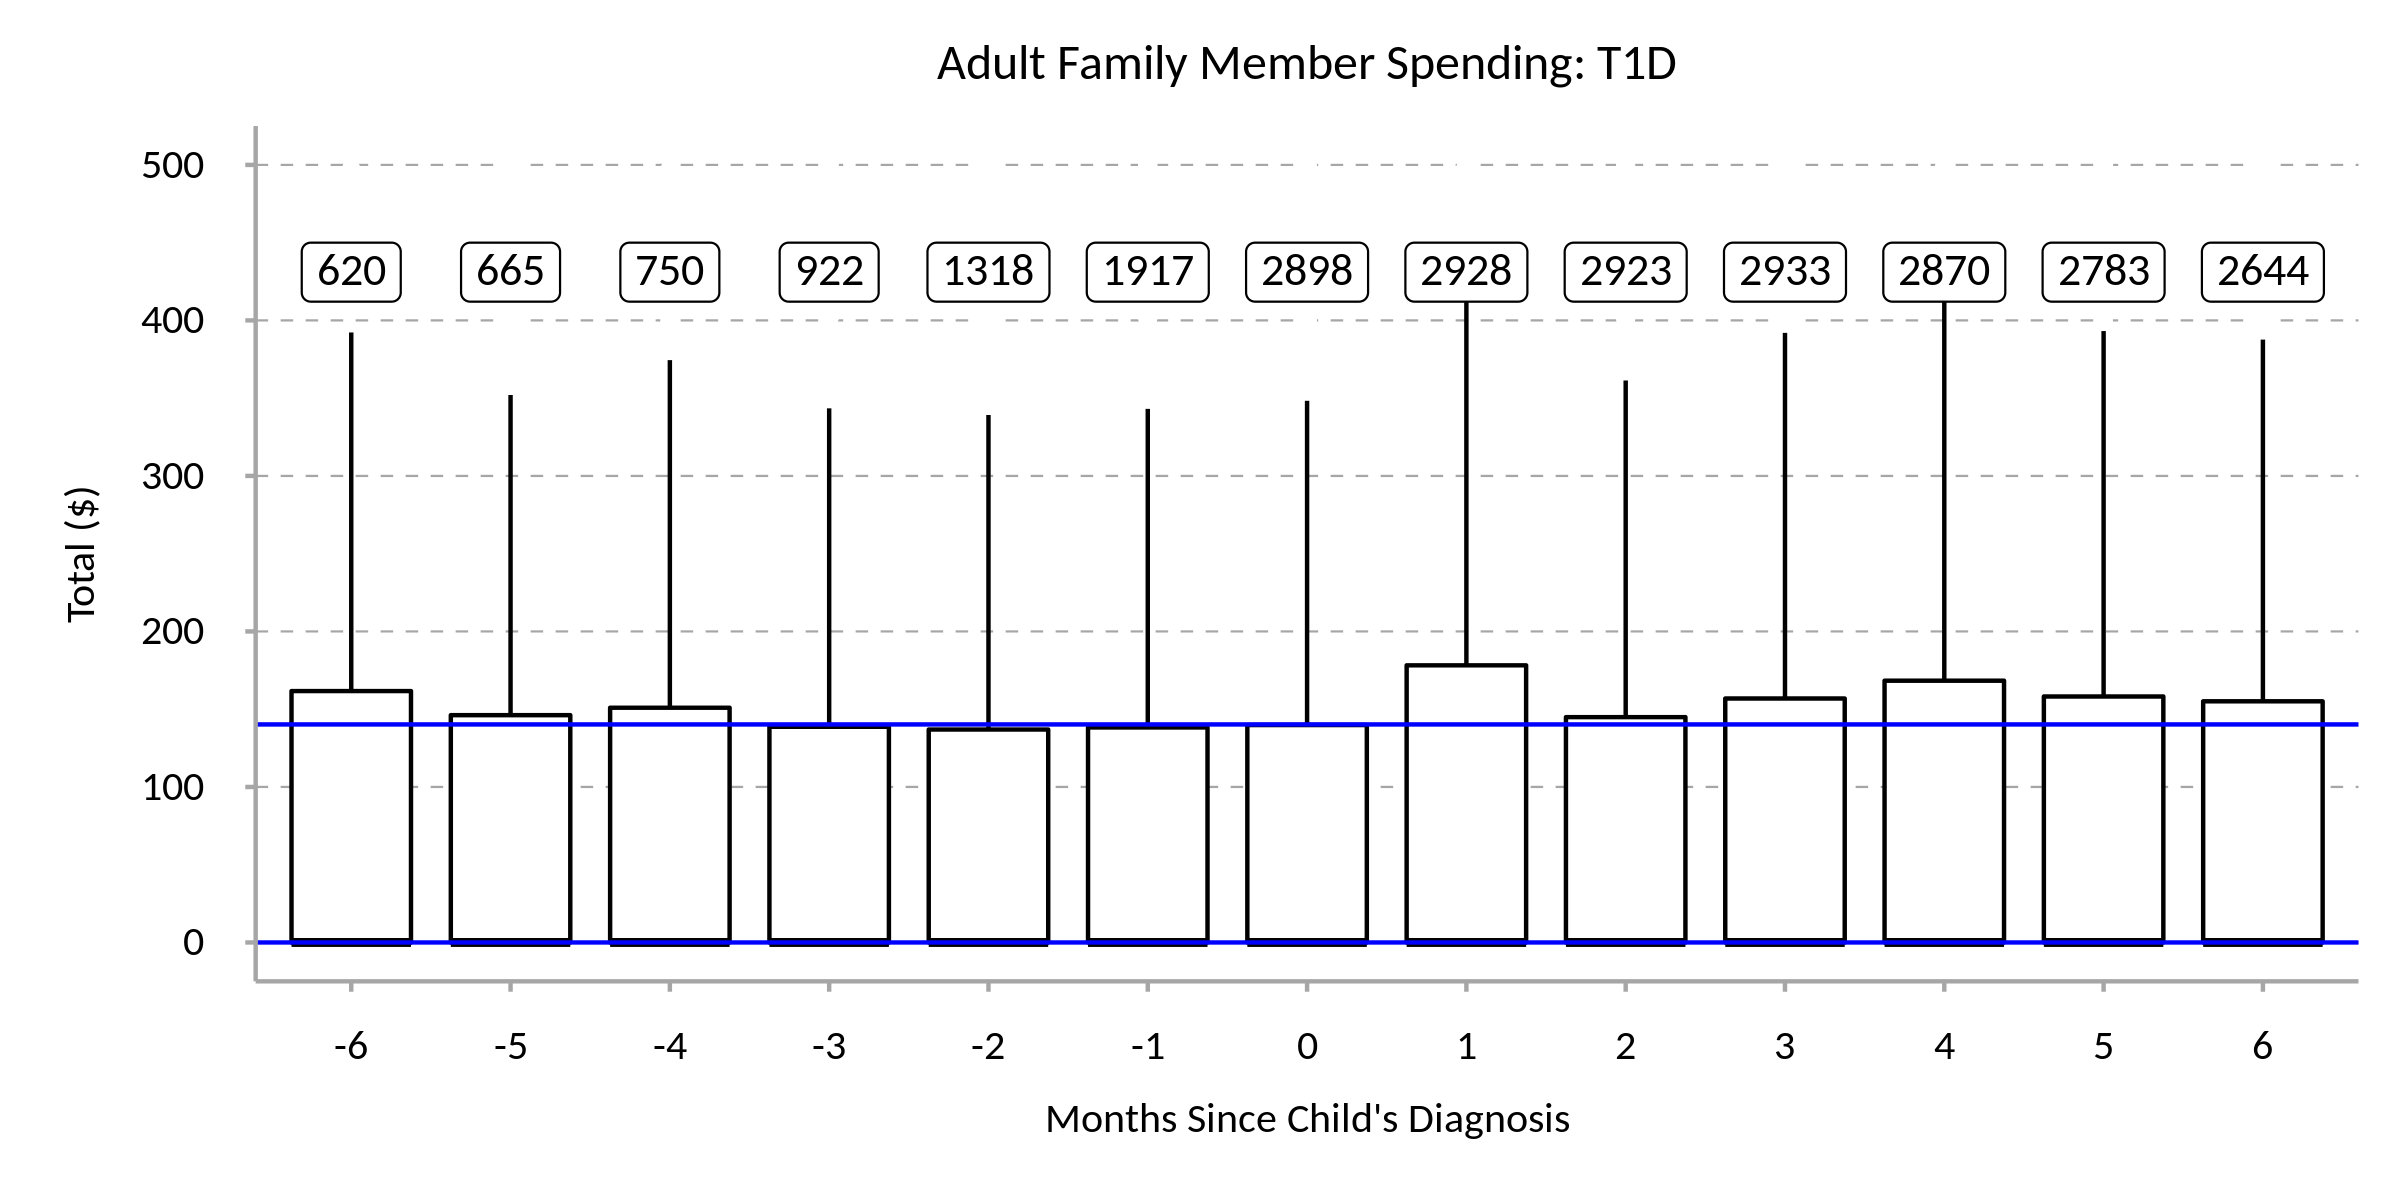
\includegraphics[width=\linewidth]{../figures/adult_family_spend_T1D.png}
\end{frame}

\begin{frame}{Trauma - Sick Child Spending}
\small
Outliers not shown. Blue lines represent median and 75 percentile of spend before diagnosis. Numbers
shown are number of member months included in boxplot. 
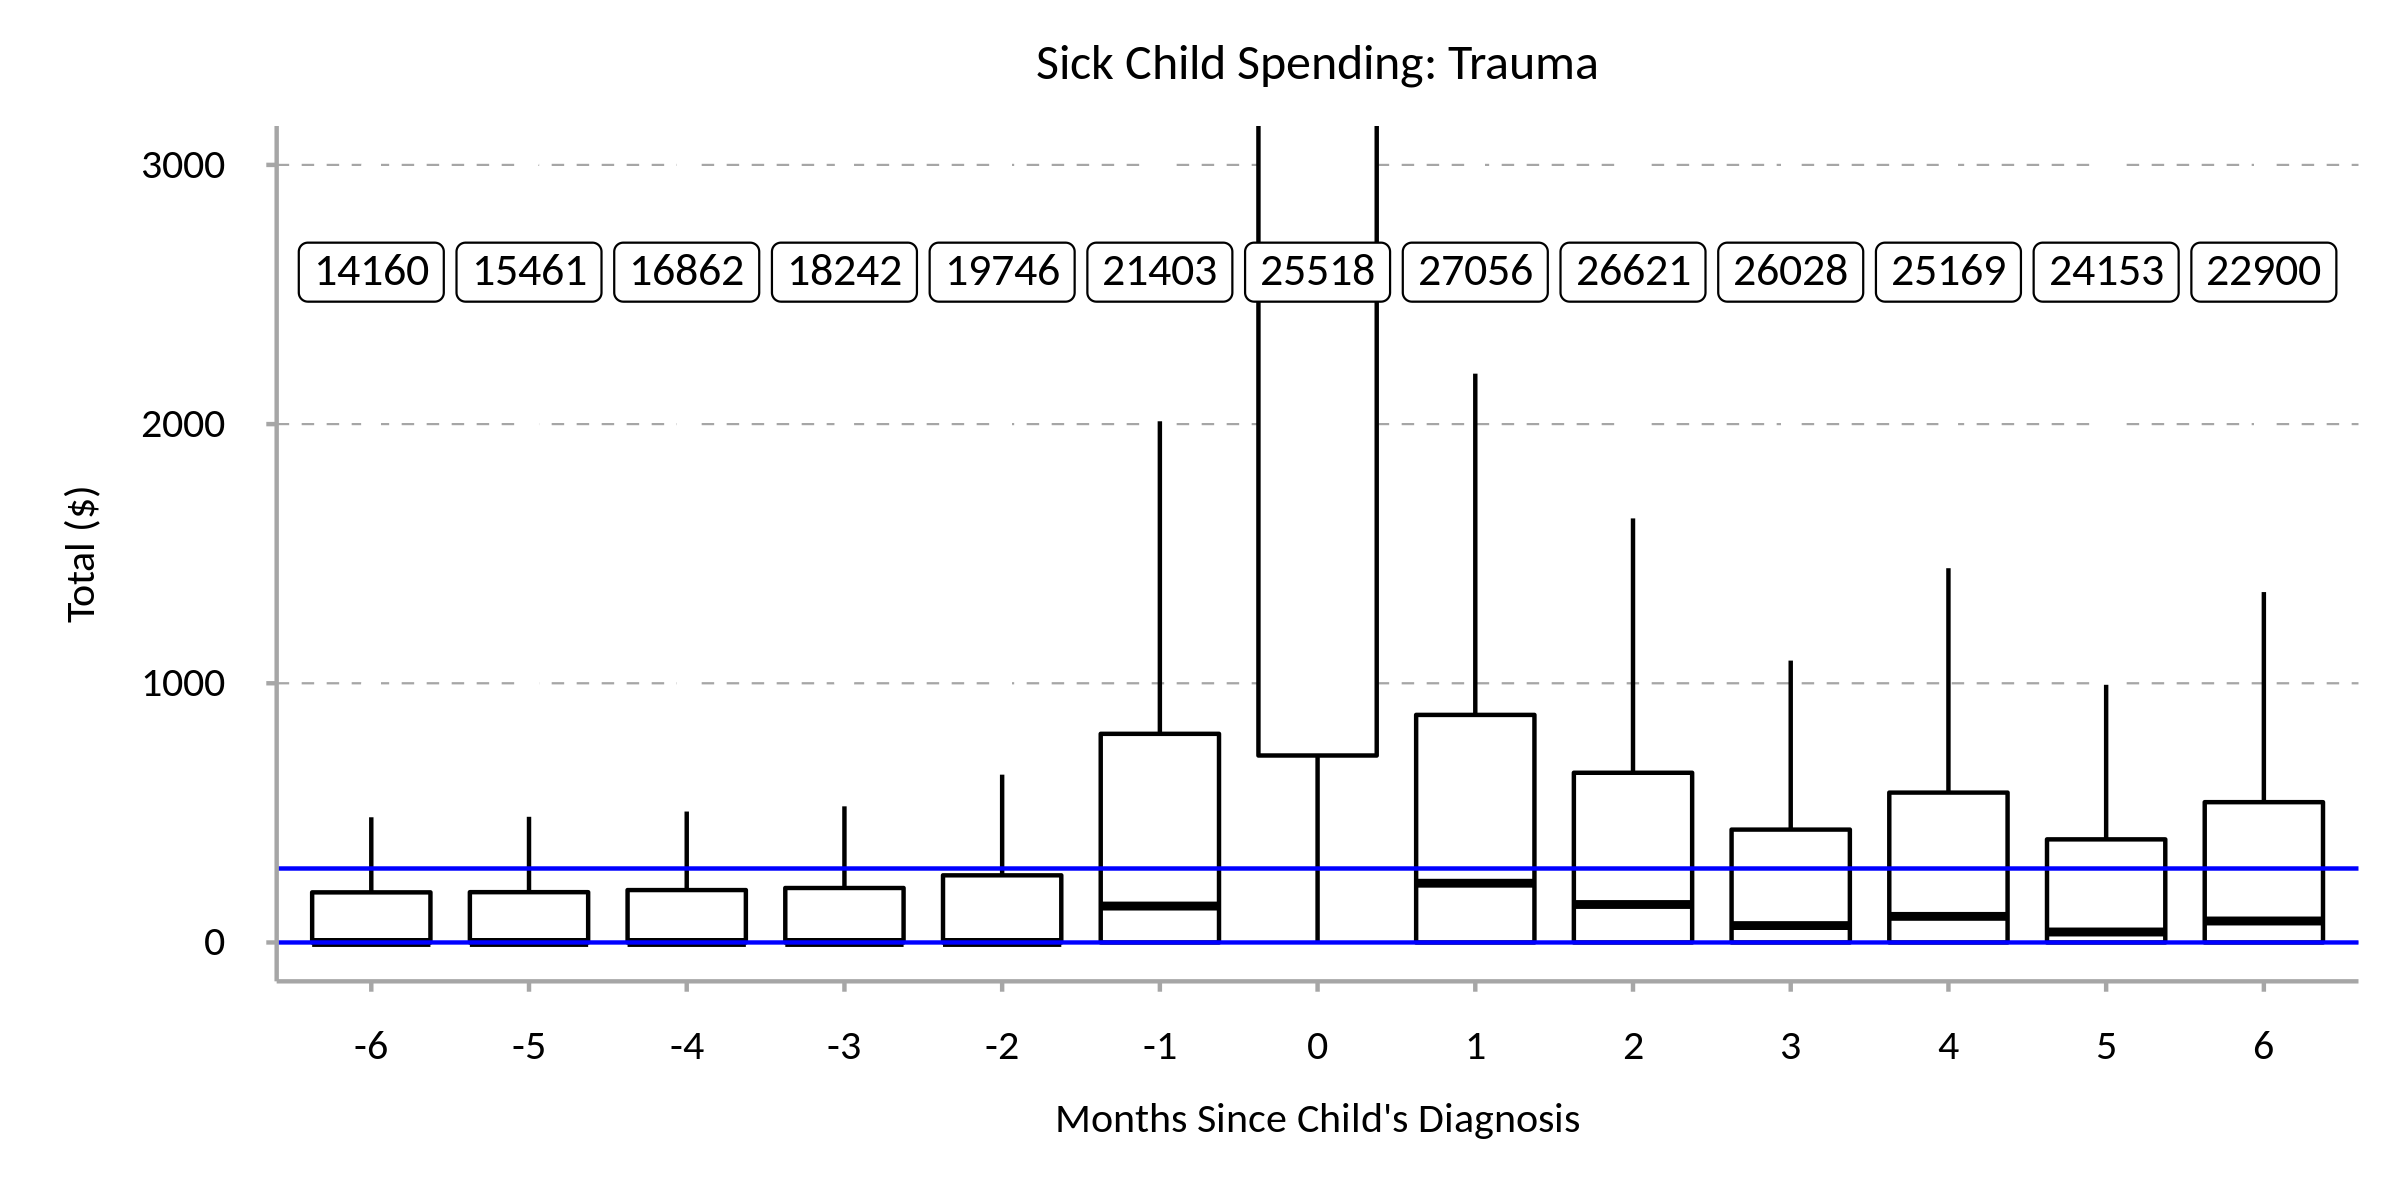
\includegraphics[width=\linewidth]{../figures/sick_child_spend_Trauma.png}
\end{frame}

\begin{frame}{Trauma - Adult Spending}
\small
Outliers not shown. Blue lines represent median and 75 percentile of spend before diagnosis. Numbers
shown are number of member months included in boxplot. 
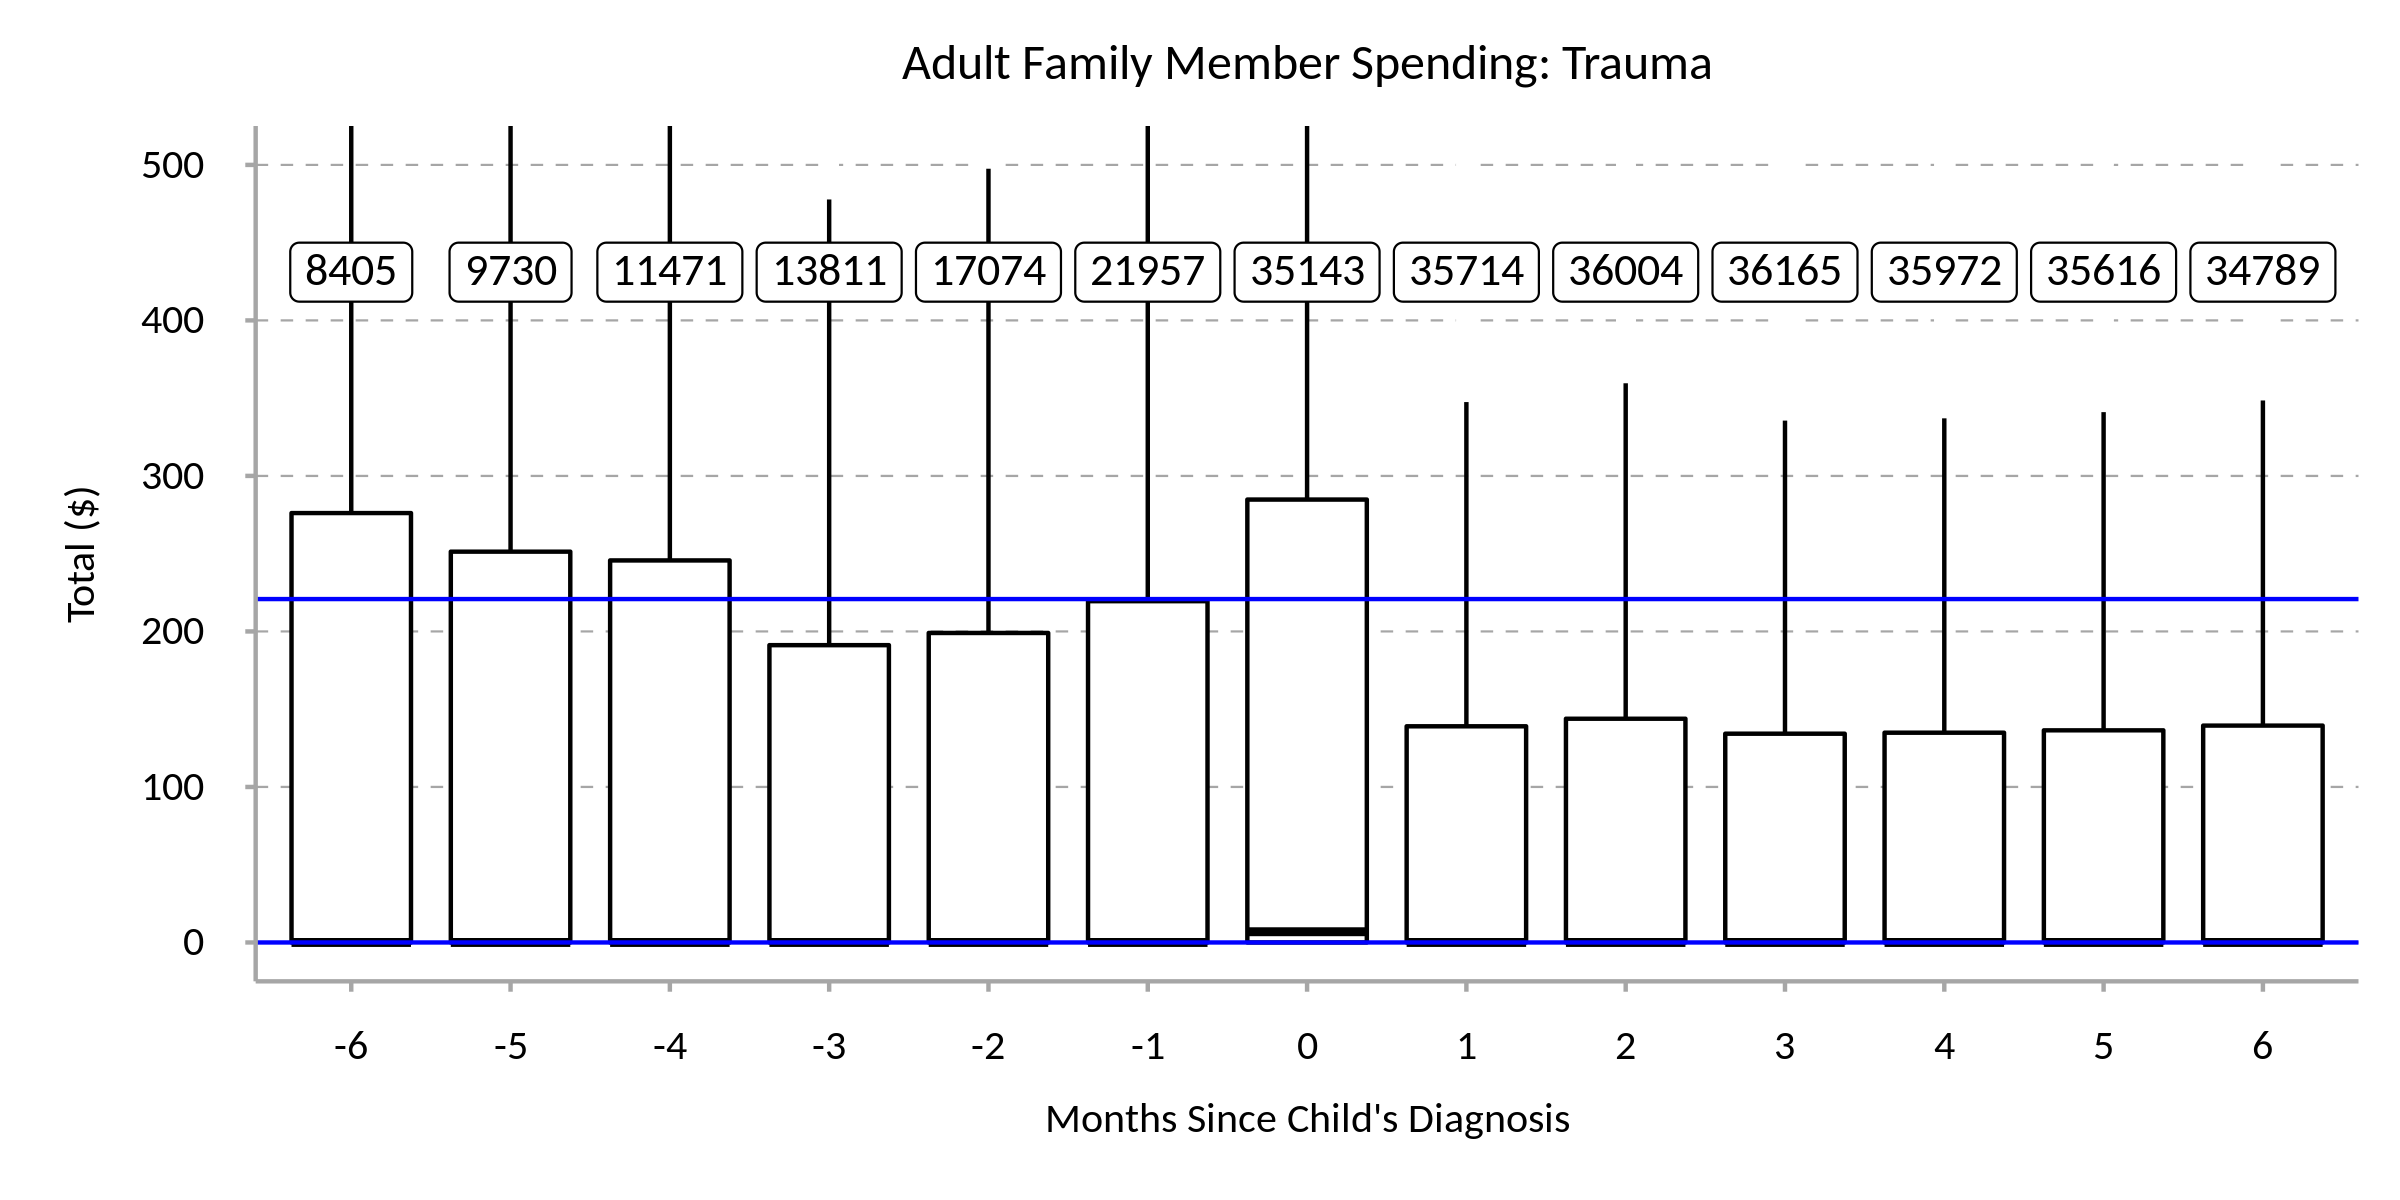
\includegraphics[width=\linewidth]{../figures/adult_family_spend_Trauma.png}
\end{frame}

\section{\scshape Modeling}

\begin{frame}{Initial Model}
\begin{itemize}
	\item Calculated average monthly spend per adult family member before and after diagnosis, using data within 24 months of diagnosis. 
	\item Response: square root of average monthly spend. 
	\item Predictors: RAF, Age, Indicator of after child's diagnosis, Indicator of male, Indicator of only one adult on the plan (No other 'parents' on plan). 
	\item Scaled average RAF and Age to have mean 0 and variance 1 in order to compare size of parameter estimates. 
	\item Fit linear least squares model and linear quantile regression model looking at change in median and 75th quantile. Calculated parameter estimates and 95\% confidence intervals using 1000 bootstrap samples. 

\end{itemize}
\end{frame}

\begin{frame}{Autism diagnosis effect on adult family. }
  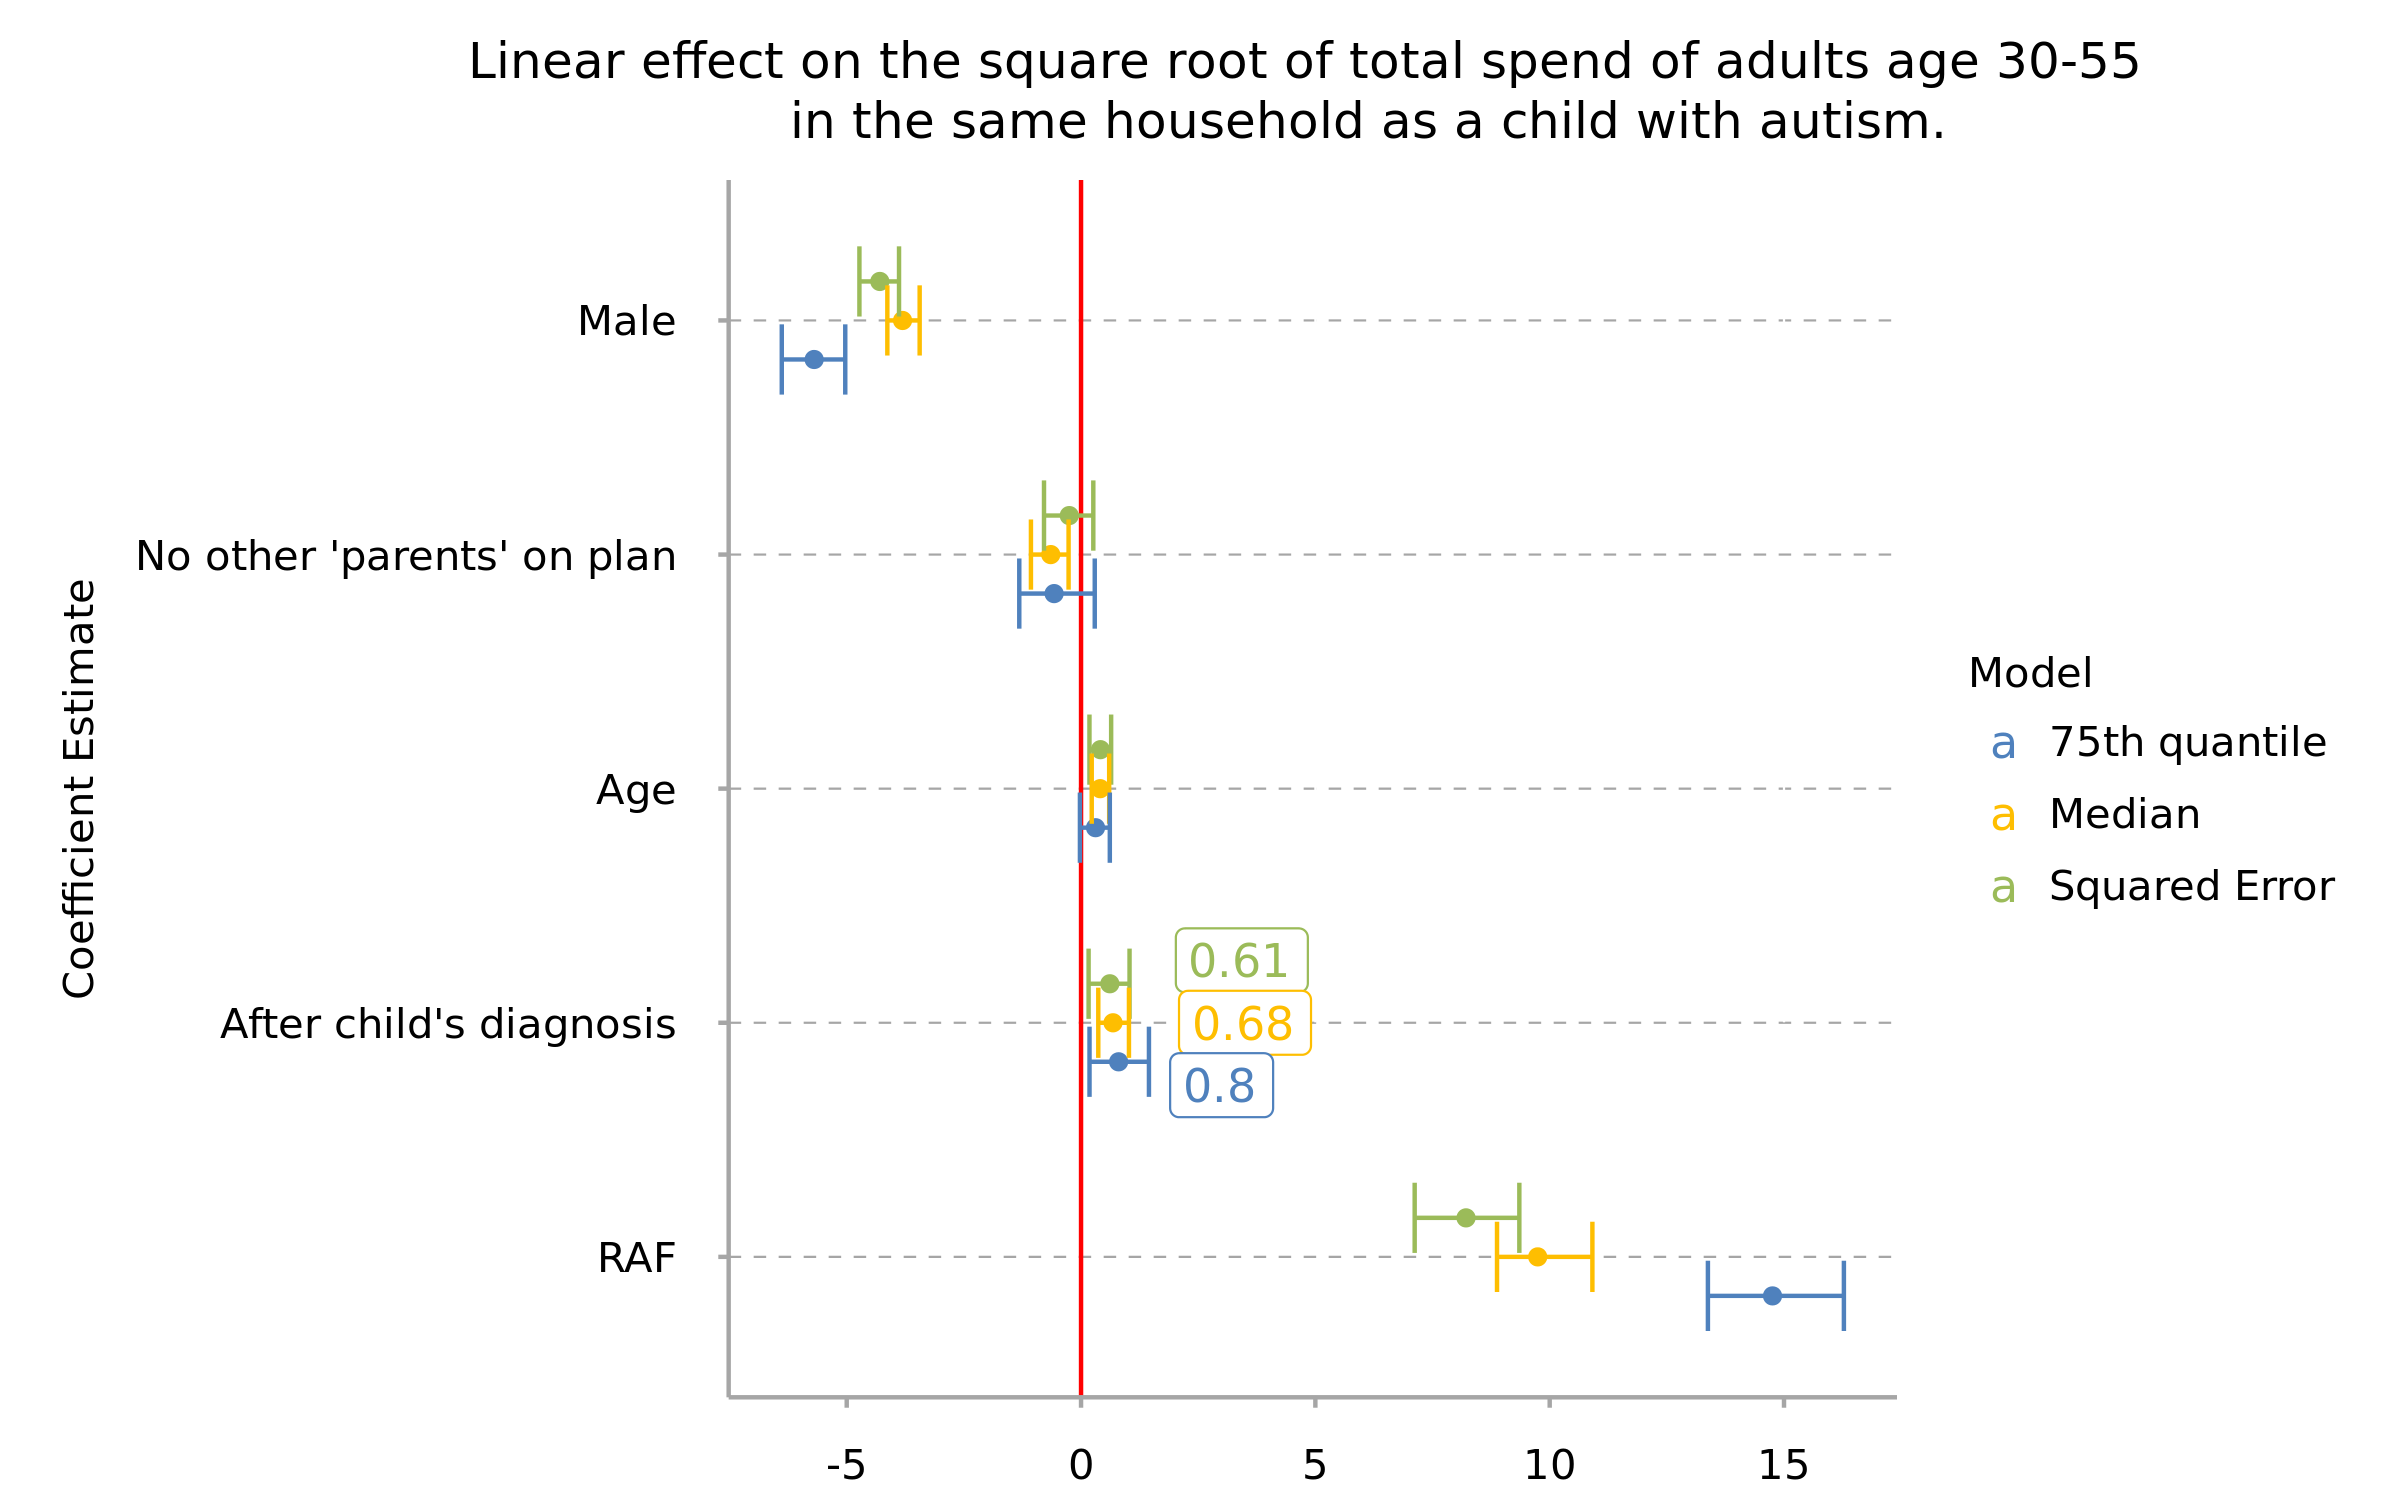
\includegraphics[width=\linewidth]{../figures/parameter_est_ASD.png}
\end{frame}

\begin{frame}{Asthma diagnosis effect on adult family. }
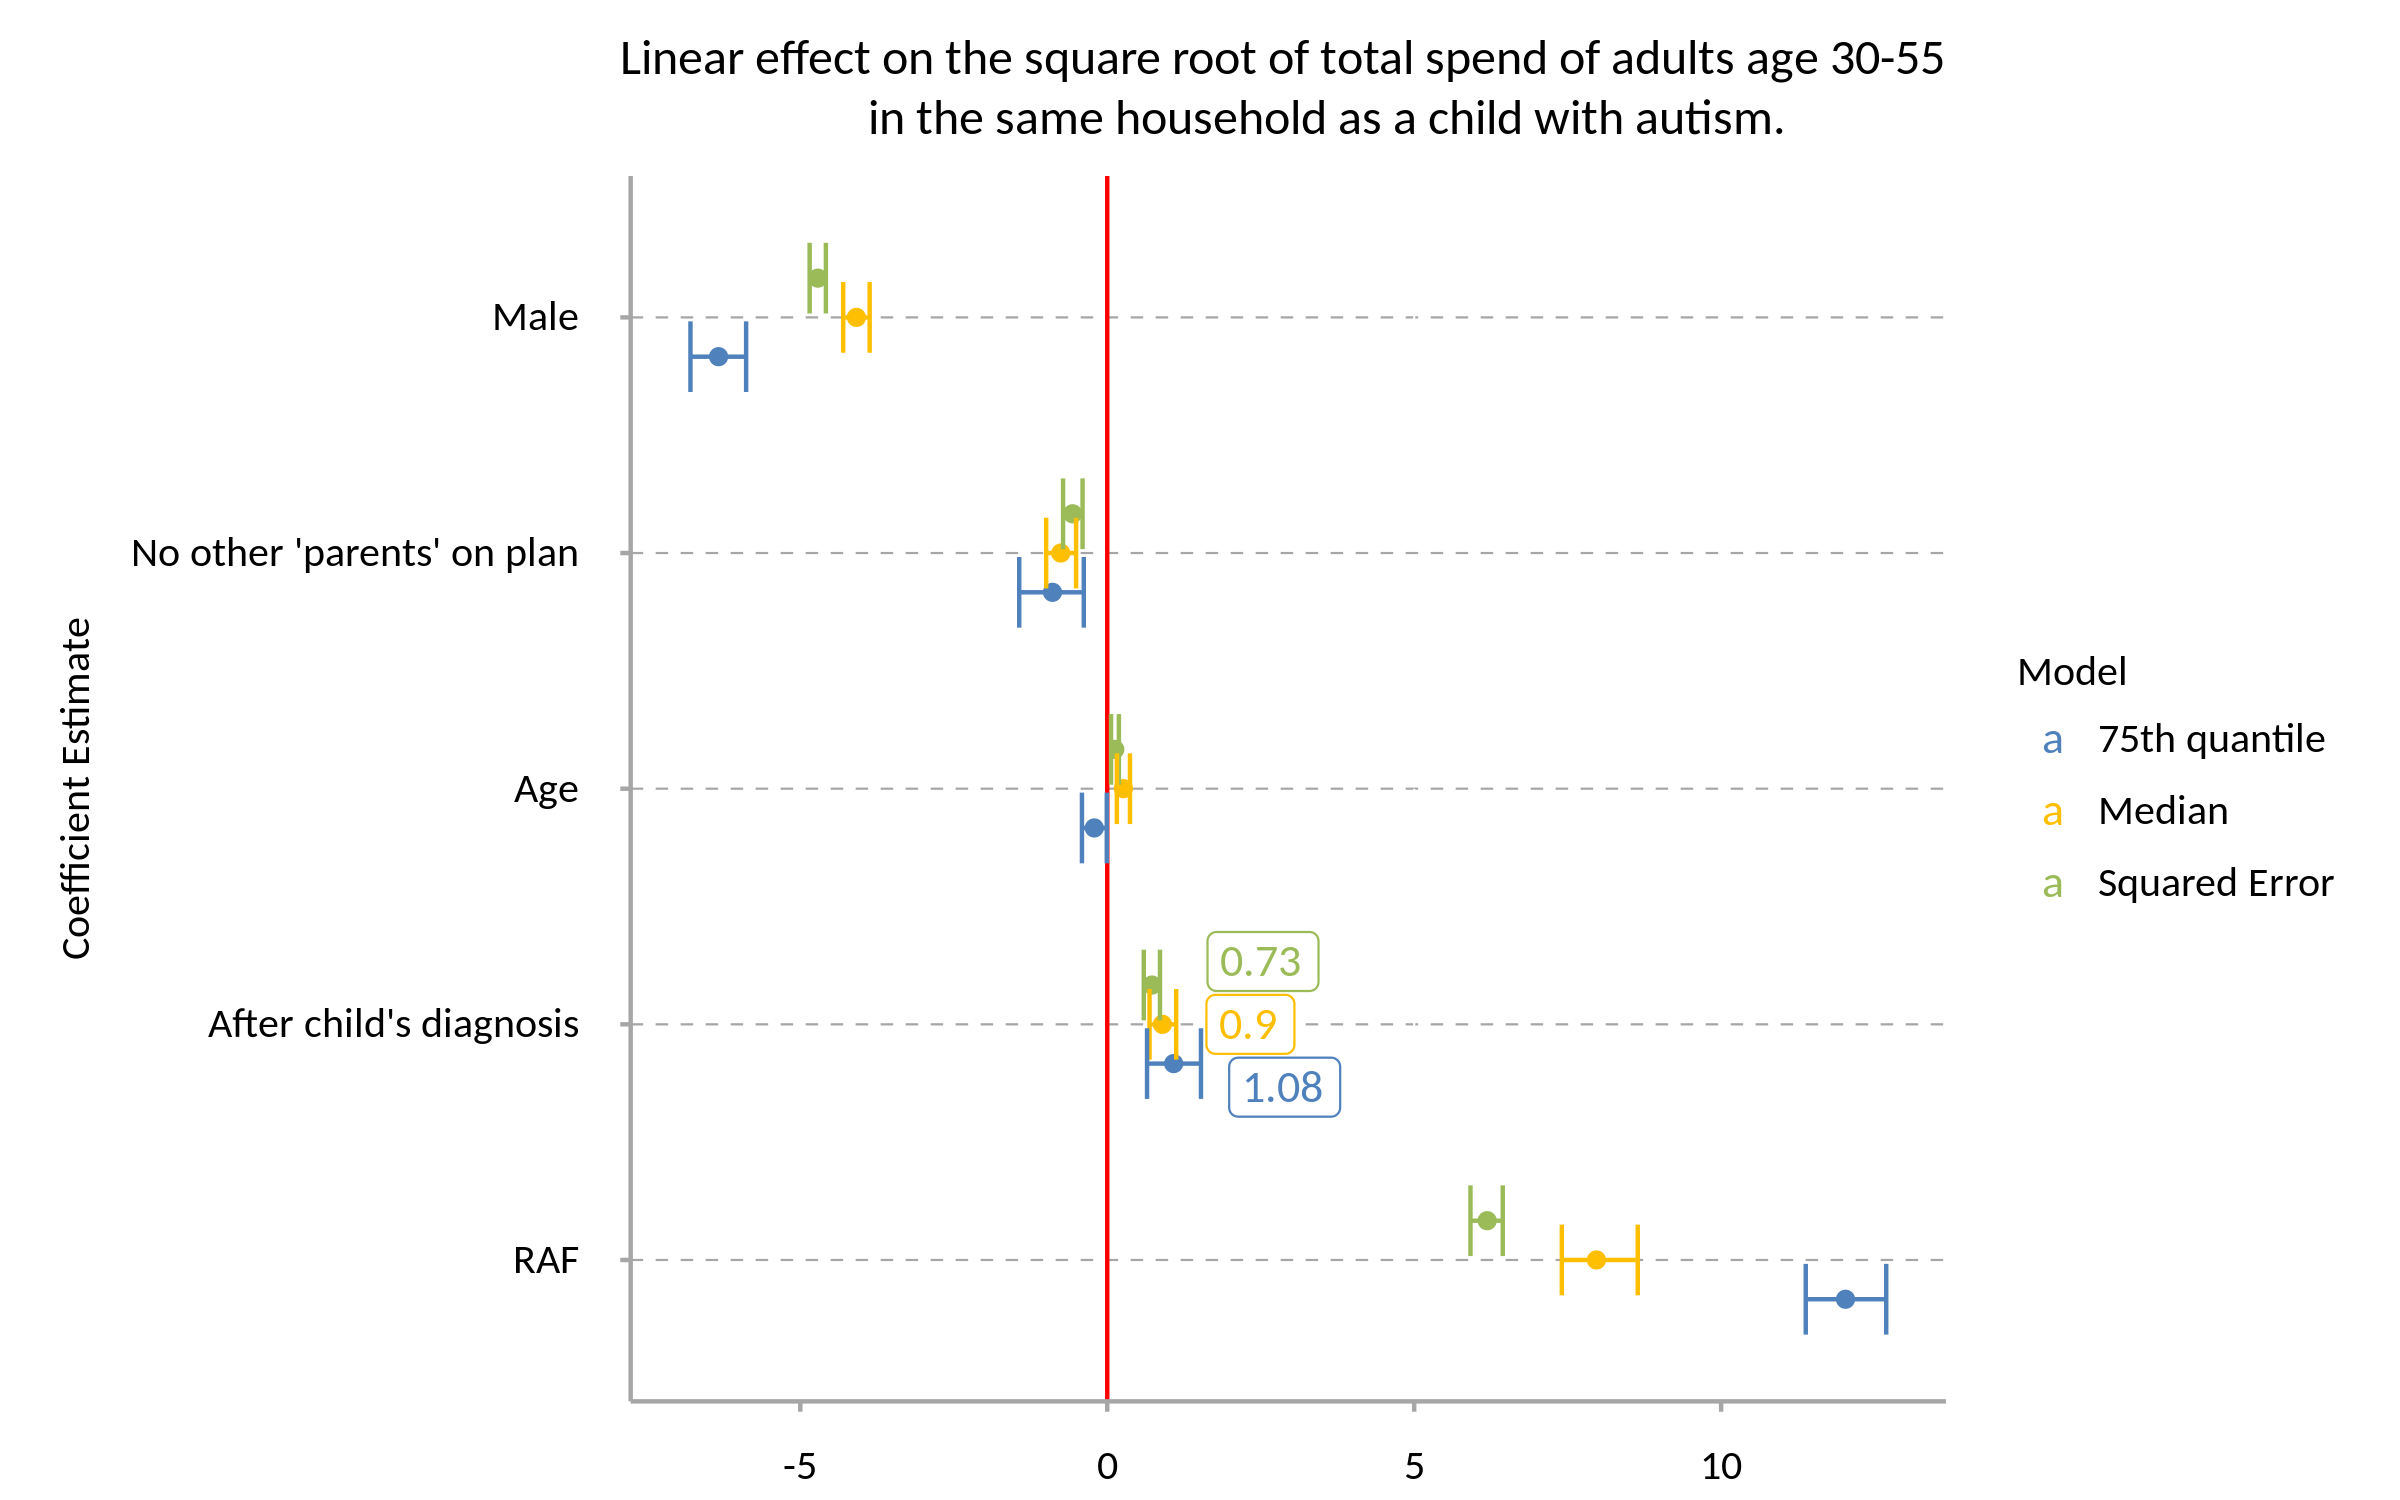
\includegraphics[width=\linewidth]{../figures/parameter_est_Asthma.png}

\center
\tiny
Quantile regression fit on sample of data (25,000), due to large size ($>100,000$)
\end{frame}

\begin{frame}{Diabetes diagnosis effect on adult family. }
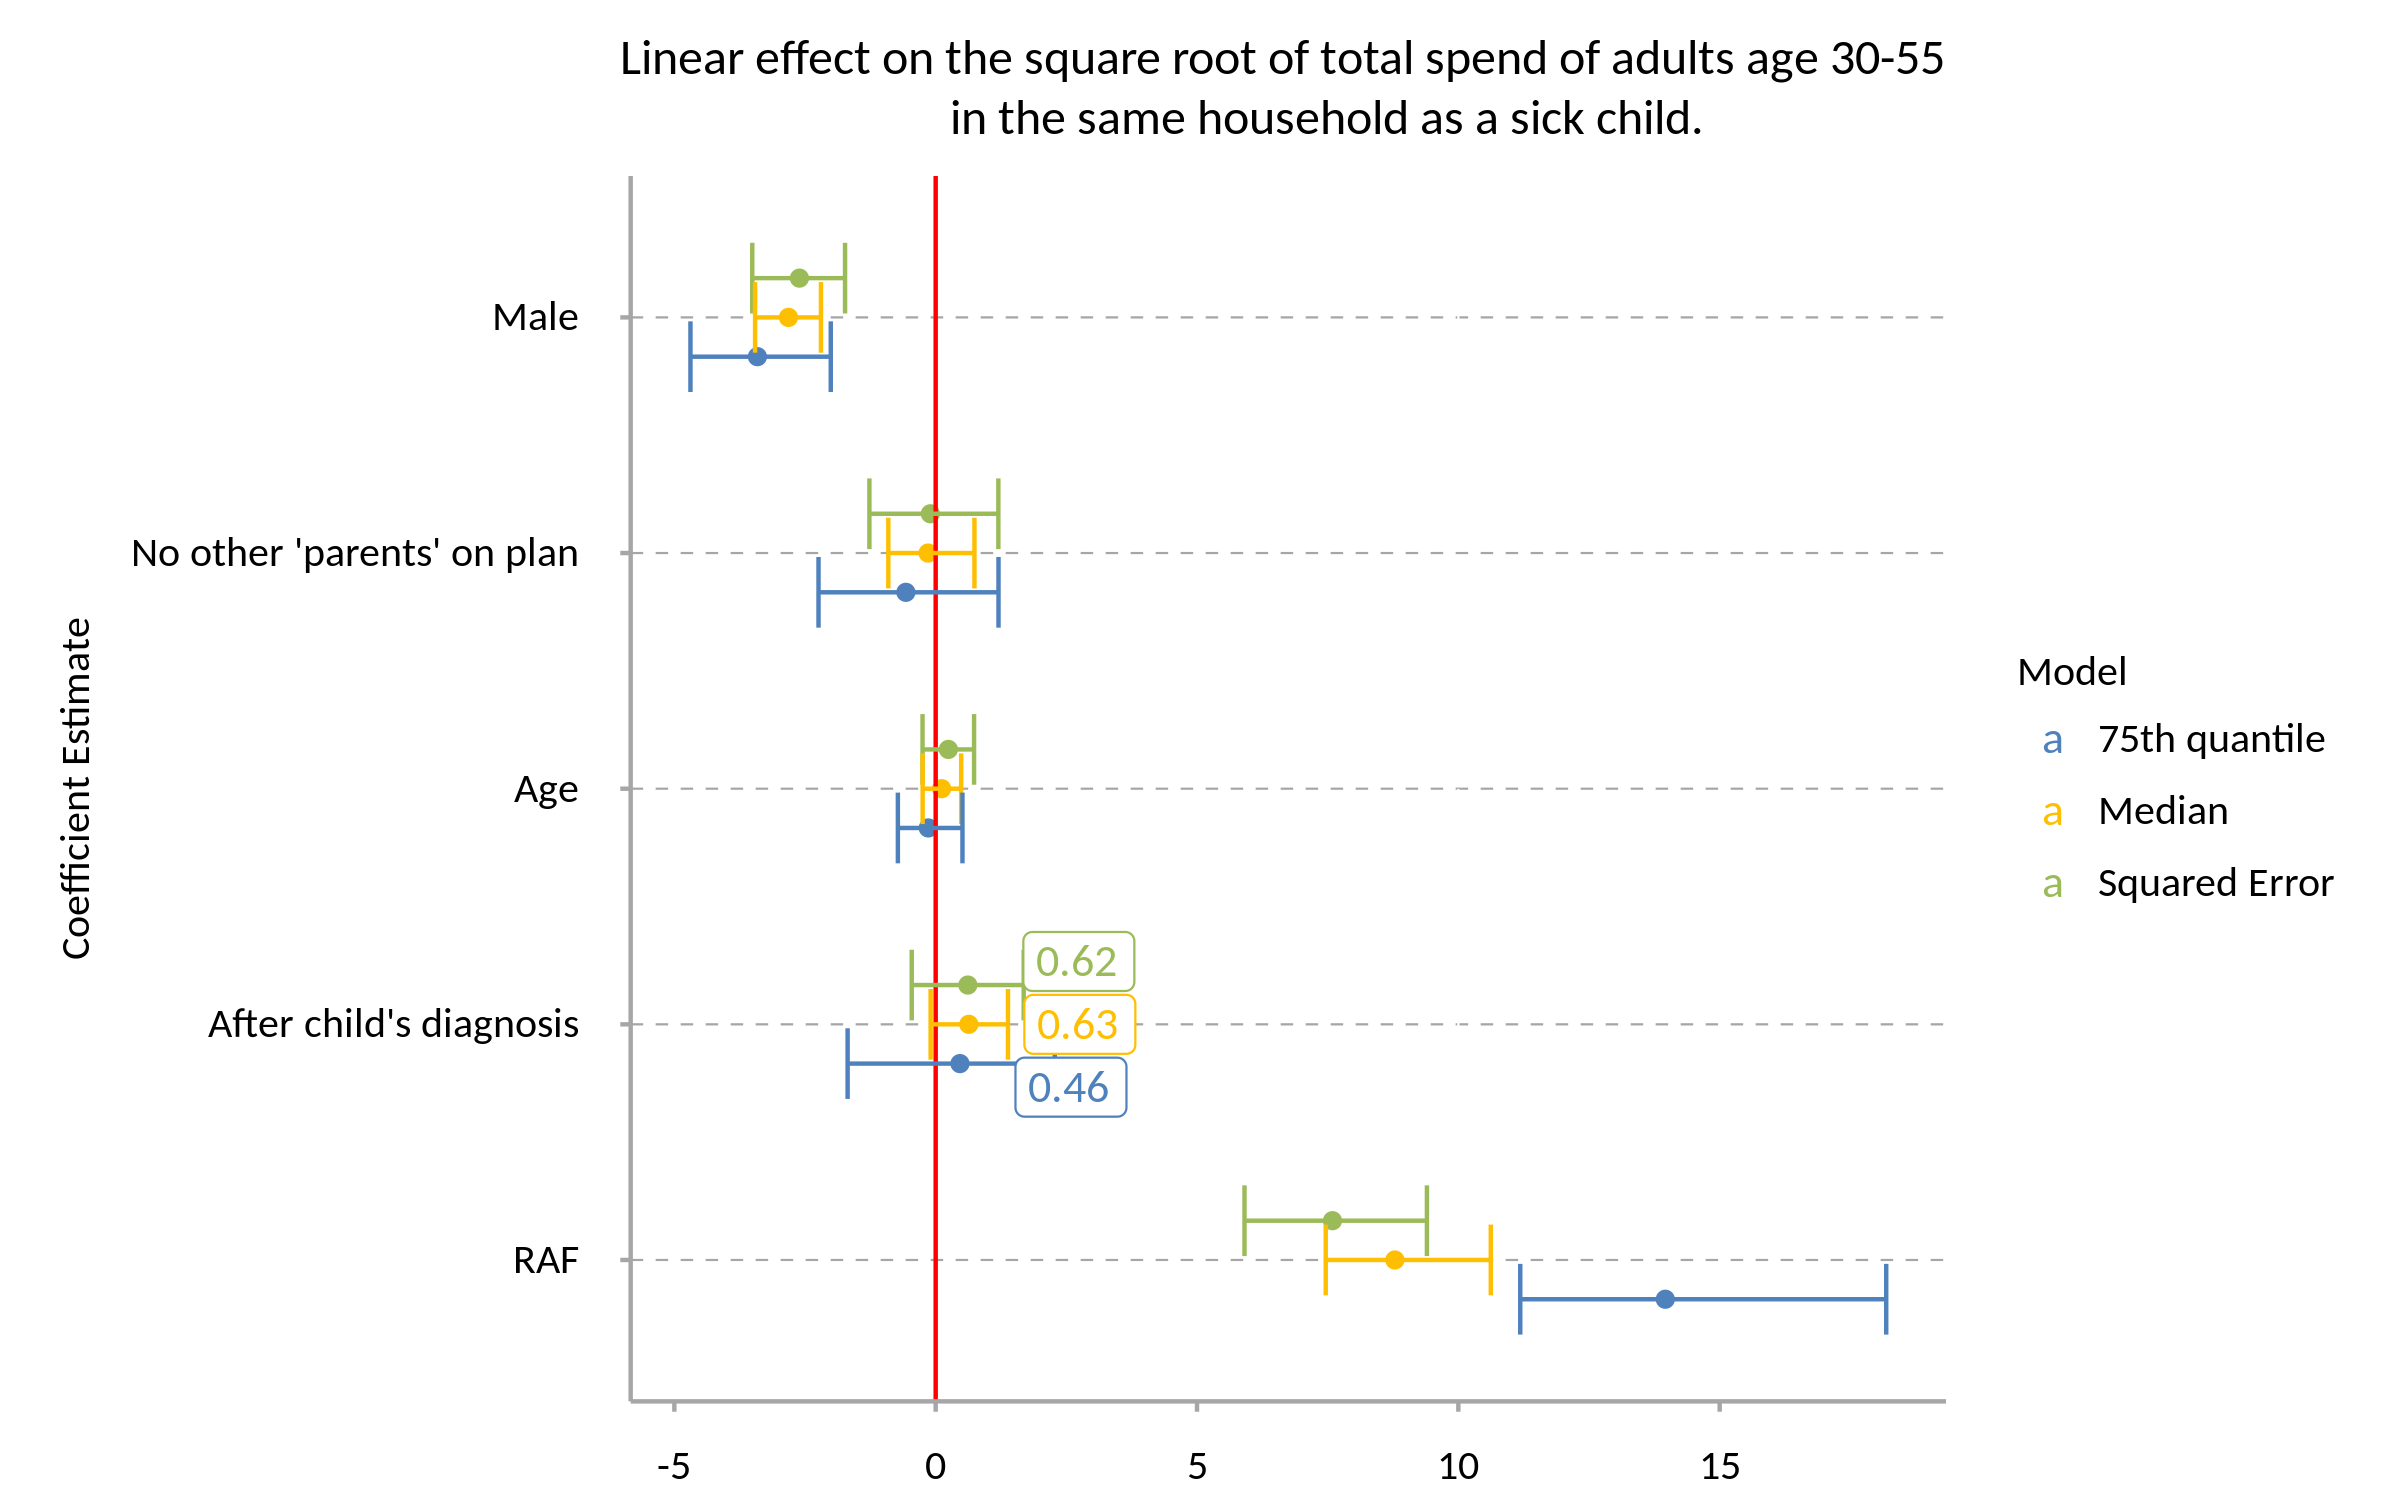
\includegraphics[width=\linewidth]{../figures/parameter_est_T1D.png}
\end{frame}

\end{document}